\documentclass[10pt]{article}
\usepackage[utf8]{inputenc}
\usepackage[T1]{fontenc}
\usepackage{amsmath}
\usepackage{amsfonts}
\usepackage{amssymb}
\usepackage[version=4]{mhchem}
\usepackage{stmaryrd}
\usepackage{graphicx}
\usepackage[export]{adjustbox}
\graphicspath{ {./images/} }

\title{The Triple Integral }

\author{}
\date{}


\begin{document}
\maketitle
Let $f(x, y, z)$ be a continuous function on a three-dimensional region $R$. The definition of the double integral can be extended in an obvious way to obtain the definition of the triple integral $\iint_{R} f(x, y, z) d V$.

If $f(x, y, z)=1$, then $\iint_{R} f(x, y, z) d V$ may be interpreted as measuring the volume of the region $R$.

\section*{Evaluation of Triple Integrals}
As in the case of double integrals, a triple integral can be evaluated in terms of iterated integrals.

In rectangular coordinates,

$$
\begin{aligned}
\iiint_{R} f(x, y, z) d V & =\int_{a}^{b} \int_{y_{1}(x)}^{y_{2}(x)} \int_{z_{1}(x, y)}^{z_{2}(x, y)} f(x, y, z) d z d y d x \\
& =\int_{c}^{d} \int_{x_{1}(y)}^{x_{2}(y)} \int_{z_{1}(x, y)}^{z_{2}(x, y)} f(x, y, z) d z d x d y, \text { etc. }
\end{aligned}
$$

where the limits of integration are chosen to cover the region $R$.

In cylindrical coordinates,

$$
\iiint_{R} f(r, \theta, z) d V=\int_{\alpha}^{\beta} \int_{r_{1}(\theta)}^{r_{2}(\theta)} \int_{z_{1}(r, \theta)}^{z_{2}(r, \theta)} f(r, \theta, z) r d z d r d \theta
$$

where the limits of integration are chosen to cover the region $R$. (See Problem 23.)

In spherical coordinates,

$$
\iiint_{R} f(\rho, \phi, \theta) d V=\int_{\alpha}^{\beta} \int_{\phi_{1}(\theta)}^{\phi_{2}(\theta)} \int_{\rho_{1}(\phi, \theta)}^{\rho_{2}(\phi, \theta)} f(\rho, \phi, \theta) \rho^{2} \sin \phi d \rho d \phi d \theta
$$

where the limits of integration are chosen to cover the region $R$. (See Problem 24.)

Discussion of the definitions: Consider the function $f(x, y, z)$, continuous over a region $R$ of ordinary space. After slicing $R$ with planes $x=\xi_{i}$ and $y=\eta_{i}$ as in Chapter 54, let these subregions be further sliced by planes $z=\zeta_{k}$. The region $R$ has now been separated into a number of rectangular parallelepipeds of volume $\Delta V_{i j k}=\Delta x_{i} \Delta y_{j} \Delta z_{k}$ and a number of partial parallelepipeds which we shall ignore. In each complete parallelepiped, select a point $P_{i j k}\left(x_{i}, y_{j}, z_{k}\right)$; then compute $f\left(x_{i}, y_{j}, z_{k}\right)$ and form the sum


\begin{equation*}
\sum_{\substack{i=1, \ldots, m \\ j=1, \ldots, n \\ k=1, \ldots, p}} f\left(x_{i}, y_{j}, z_{k}\right) \Delta V_{i j k}=\sum_{\substack{i=1, \ldots, m \\ j=1, \ldots, n \\ k=1, \ldots, p}} f\left(x_{i}, y_{j}, z_{k}\right) \Delta x_{i} \Delta y_{j} \Delta z_{k} \tag{57.1}
\end{equation*}


The triple integral of $f(x, y, z)$ over the region $R$ is defined to be the limit of (57.1) as the number of parallelepipeds is indefinitely increased in such a manner that all dimensions of each go to zero.

In evaluating this limit, we may sum first each set of parallelepipeds having $\Delta_{i} x$ and $\Delta_{j} y$, for fixed $i$ and $j$, as two dimensions and consider the limit as each $\Delta_{k} z \rightarrow 0$. We have

$$
\lim _{p \rightarrow+\infty} \sum_{k=1}^{p} f\left(x_{i}, y_{i}, z_{k}\right) \Delta_{k} z \Delta_{i} x \Delta_{j} y=\int_{z_{1}}^{z_{2}} f\left(x_{i}, y_{i}, z\right) d z \Delta_{i} x \Delta_{j} y
$$

Now these are the columns, the basic subregions, of Chapter 54; hence,

$$
\lim _{\substack{m \rightarrow+\infty \\ n \rightarrow+\infty \\ p \rightarrow+\infty \\ p \rightarrow+1, \ldots, n \\ k=1, \ldots, n}} \sum_{\substack{i=1 \\ k=1, \ldots}} f\left(x_{i}, y_{j}, z_{k}\right) \Delta V_{i j k}=\iiint_{R} f(x, y, z) d z d x d y=\iiint_{R} f(x, y, z) d z d y d x
$$

\section*{Centroids and Moments of Inertia}
The coordinates $(\bar{x}, \bar{y}, \bar{z})$ of the centroid of a volume satisfy the relations

$$
\bar{x} \iiint_{R} d V=\iiint_{R} x d V, \quad \bar{y} \iiint_{R} d V=\iiint_{R} y d V, \quad \bar{z} \iiint_{R} d V=\iiint_{R} z d V
$$

The moments of inertia of a volume with respect to the coordinate axes are given by

$$
I_{x}=\iiint_{R}\left(y^{2}+z^{2}\right) d V, \quad I_{y}=\iiint_{R}\left(z^{2}+x^{2}\right) d V, \quad I_{z}=\iiint_{R}\left(x^{2}+y^{2}\right) d V
$$

\section*{SOLVED PROBLEMS}
\begin{enumerate}
  \item Evaluate the given triple integrals:
\end{enumerate}

(a) $\int_{0}^{1} \int_{0}^{1-x} \int_{0}^{2-x} x y z d z d y d x$

$$
\begin{aligned}
& =\int_{0}^{1}\left[\int_{0}^{1-x}\left(\int_{0}^{2-x} x y z d z\right) d y\right] d x \\
& =\int_{0}^{1}\left[\int_{0}^{1-x}\left(\left.\frac{x y z^{2}}{2}\right|_{z=0} ^{z=2-x}\right) d y\right] d x=\int_{0}^{1}\left[\int_{0}^{1-x} \frac{x y(2-x)^{2}}{2} d y\right] d x \\
& =\int_{0}^{1}\left[\frac{x y^{2}(2-x)^{2}}{4}\right]_{y=0}^{y=1-x} d x=\frac{1}{4} \int_{0}^{1}\left(4 x-12 x^{2}+13 x^{3}-6 x^{4}+x^{5}\right) d x=\frac{13}{240}
\end{aligned}
$$

(b) $\int_{0}^{\pi / 2} \int_{0}^{1} \int_{0}^{2} z r^{2} \sin \theta d z d r d \theta$

$$
\begin{aligned}
& =\int_{0}^{\pi / 2} \int_{0}^{1}\left[\frac{z^{2}}{2}\right]_{0}^{2} r^{2} \sin \theta d r d \theta=2 \int_{0}^{\pi / 2} \int_{0}^{1} r^{2} \sin \theta d r d \theta \\
& =\frac{2}{3} \int_{0}^{\pi / 2}\left[r^{3}\right]_{0}^{1} \sin \theta d \theta=-\frac{2}{3}[\cos \theta]_{0}^{\pi / 2}=\frac{2}{3}
\end{aligned}
$$

(c) $\int_{0}^{\pi} \int_{0}^{\pi / 4} \int_{0}^{\sec \phi} \sin 2 \phi d \rho d \phi d \theta$

$$
=2 \int_{0}^{\pi} \int_{0}^{\pi / 4} \sin \phi d \phi d \theta=2 \int_{0}^{\pi}\left(1-\frac{1}{2} \sqrt{2}\right) d \theta=(2-\sqrt{2}) \pi
$$

\begin{enumerate}
  \setcounter{enumi}{1}
  \item Compute the triple integral of $F(x, y, z)=z$ over the region $R$ in the first octant bounded by the planes $y=0$, $z=0, x+y=2,2 y+x=6$, and the cylinder $y^{2}+z^{2}=4$. (See Fig. 57-3.)
\end{enumerate}

Integrate first with respect to $z$ from $z=0$ (the $x y$ plane) to $z=\sqrt{4-y^{2}}$ (the cylinder), then with respect to $x$ from $x=2-y$ to $x=6-2 y$, and finally with respect to $y$ from $y=0$ to $y=2$. This yields

$$
\begin{aligned}
\iiint_{R} z d V & =\int_{0}^{2} \int_{2-y}^{6-2 y} \int_{0}^{\sqrt{4-y^{2}}} z d z d x d y=\int_{0}^{2} \int_{2-y}^{6-2 y}\left[\frac{1}{2} z^{2}\right]_{0}^{\sqrt{4-y^{2}}} d x d y \\
& =\frac{1}{2} \int_{0}^{2} \int_{2-y}^{6-2 y}\left(4-y^{2}\right) d x d y=\frac{1}{2} \int_{0}^{2}\left[\left(4-y^{2}\right) x\right]_{2-y}^{6-2 y} d y=\frac{26}{3}
\end{aligned}
$$

\begin{center}
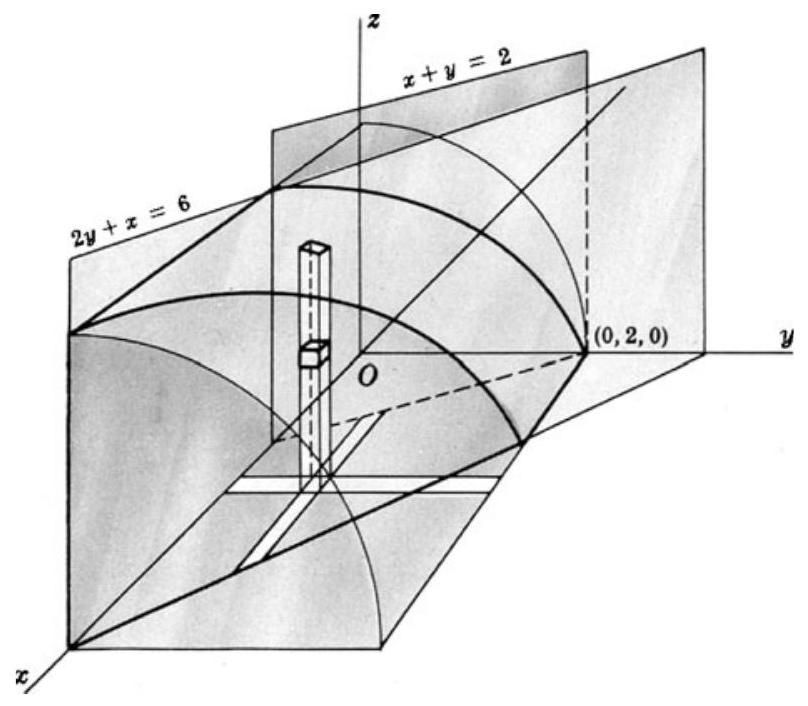
\includegraphics[max width=\textwidth]{2024_04_20_fe2e8e718cc0fcd63d1bg-03(1)}
\end{center}

Fig. 57-3

\begin{enumerate}
  \setcounter{enumi}{2}
  \item Compute the triple integral of $f(r, \theta, \mathrm{z})=r^{2}$ over the region $R$ bounded by the paraboloid $r^{2}=9-z$ and the plane $z=0$. (See Fig. 57-4.)
\end{enumerate}

\begin{center}
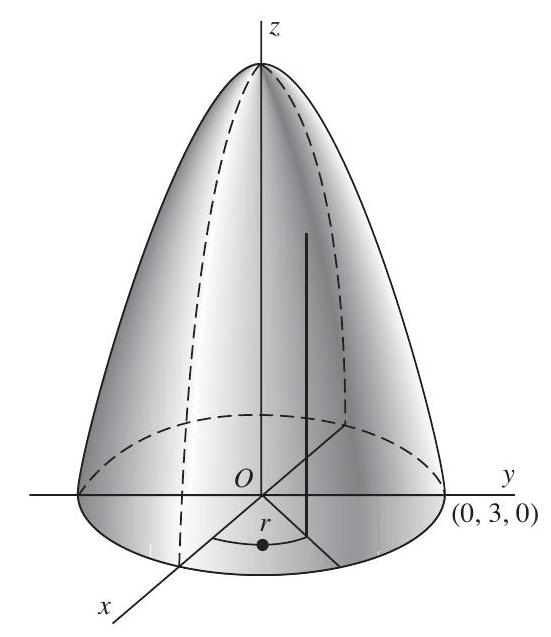
\includegraphics[max width=\textwidth]{2024_04_20_fe2e8e718cc0fcd63d1bg-03}
\end{center}

Fig. 57-4

Integrate first with respect to $z$ from $z=0$ to $z=9-r^{2}$, then with respect to $r$ from $r=0$ to $r=3$, and finally with respect to $\theta$ from $\theta=0$ to $\theta=2 \pi$. This yields

$$
\begin{aligned}
\iiint_{R} r^{2} d V & =\int_{0}^{2 \pi} \int_{0}^{3} \int_{0}^{9-r^{2}} r^{2}(r d z d r d \theta)=\int_{0}^{2 \pi} \int_{0}^{3} r^{3}\left(9-r^{2}\right) d r d \theta \\
& =\int_{0}^{2^{\pi}}\left[\frac{9}{4} r^{4}-\frac{1}{6} r^{6}\right]_{0}^{3} d \theta=\int_{0}^{2 \pi} \frac{243}{4} d \theta=\frac{243}{2} \pi
\end{aligned}
$$

\begin{enumerate}
  \setcounter{enumi}{3}
  \item Show that the following integrals give the same volume: (a) $4 \int_{0}^{4} \int_{0}^{\sqrt{16-x^{2}}} \int_{\left(x^{2}+y^{2}\right) / 4}^{4} d z d y d x$, (b) $\int_{0}^{4} \int_{0}^{2 \sqrt{z}} \int_{0}^{\sqrt{4 z-x^{2}}} d y d x d z$; and (c) $4 \int_{0}^{4} \int_{y^{2} / 4}^{4} \int_{0}^{\sqrt{4 z-y^{2}}} d x d z d y$.\\
(a) Here $z$ ranges from $z=\frac{1}{4}\left(x^{2}+y^{2}\right)$ to $z=4$, that is, the volume is bounded below by the paraboloid $4 z=x^{2}+y^{2}$ and above by the plane $z=4$. The ranges of $y$ and $x$ cover a quadrant of the circle $x^{2}+y^{2}=16, z$ $=0$, the projection of the curve of intersection of the paraboloid and the plane $z=4$ on the $x y$ plane. Thus, the integral gives the volume cut from the paraboloid by the plane $z=4$.
\end{enumerate}

(b) Here $y$ ranges from $y=0$ to $y=\sqrt{4 z-x^{2}}$, that is, the volume is bounded on the left by the $x z$ plane and on the right by the paraboloid $y^{2}=4 z-x^{2}$. The ranges of $x$ and $z$ cover one-half the area cut from the parabola $x^{2}=4 z, y=0$, the curve of intersection of the paraboloid and the $x z$ plane, by the plane $z=4$. The region $R$ is that of (a).

(c) Here the volume is bounded behind by the $y z$ plane and in front by the paraboloid $4 z=x^{2}+y^{2}$. The ranges of $z$ and $y$ cover one-half the area cut from the parabola $y^{2}=4 z, x=0$, the curve of intersection of the paraboloid and the $y z$ plane, by the plane $z=4$. The region $R$ is that of (a).

\begin{enumerate}
  \setcounter{enumi}{4}
  \item Compute the triple integral of $F(\rho, \theta, \phi)=1 / \rho$ over the region $R$ in the first octant bounded by the cones $\phi=\frac{\pi}{4}$ and $\phi=\tan ^{-1} 2$ and the sphere $\rho=\sqrt{6}$. (See Fig. 57-5.)
\end{enumerate}

\begin{center}
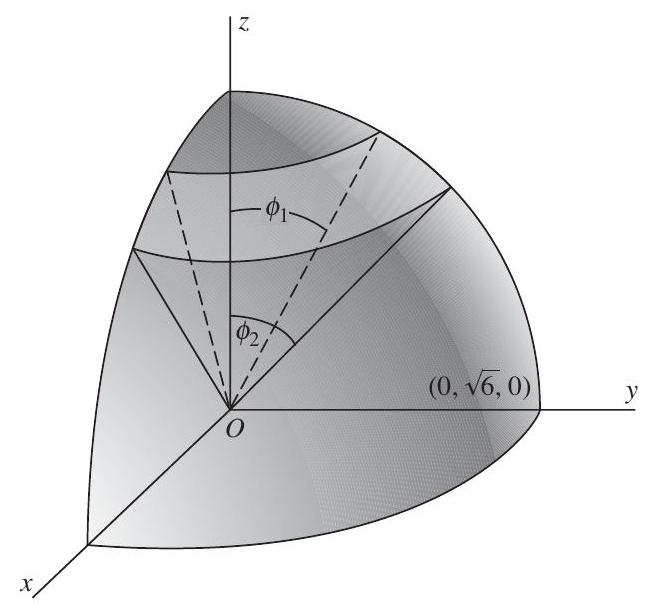
\includegraphics[max width=\textwidth]{2024_04_20_fe2e8e718cc0fcd63d1bg-04}
\end{center}

Fig. 57-5

Integrate first with respect to $\rho$ from $\rho=0$ to $\rho=\sqrt{6}$, then with respect to $\phi$ from $\phi=\frac{\pi}{4}$ to $\phi=\tan ^{-1} 2$, and finally with respect to $\theta$ from 0 to $\frac{\pi}{2}$. This yields

$$
\begin{aligned}
\iiint_{R} \frac{1}{\rho} d V & =\int_{0}^{\pi / 2} \int_{\pi / 4}^{\tan ^{-1} 2} \int_{0}^{\sqrt{6}} \frac{1}{\rho} \rho^{2} \sin \phi d \rho d \phi d \theta \\
& =3 \int_{0}^{\pi / 2} \int_{\pi / 4}^{\tan ^{-1} 2} \sin \phi d \phi d \theta \\
& =-3 \int_{0}^{\pi / 2}\left(\frac{1}{\sqrt{5}}-\frac{1}{\sqrt{2}}\right) d \theta=\frac{3 \pi}{2}\left(\frac{1}{\sqrt{2}}-\frac{1}{\sqrt{5}}\right)
\end{aligned}
$$

\begin{enumerate}
  \setcounter{enumi}{5}
  \item Find the volume bounded by the paraboloid $z=2 x^{2}+y^{2}$ and the cylinder $z=4-y^{2}$. (See Fig. 57-6.)
\end{enumerate}

Integrate first with respect to $z$ from $z=2 x^{2}+y^{2}$ to $z=4-y^{2}$, then with respect to $y$ from $y=0$ to $y=\sqrt{2-x^{2}}$ (obtain $x^{2}+y^{2}=2$ by eliminating $x$ between the equations of the two surfaces), and finally with respect to $x$ from $x=0$ to $x=\sqrt{2}$ (obtained by setting $y=0$ in $x^{2}+y^{2}=2$ ) to obtain one-fourth of the required volume. Thus,

$$
\begin{aligned}
V & =4 \int_{0}^{\sqrt{2}} \int_{0}^{\sqrt{2-x^{2}}} \int_{2 x^{2}+y^{2}}^{4-y^{2}} d z d y d x=4 \int_{0}^{\sqrt{2}} \int_{0}^{\sqrt{2-x^{2}}}\left[\left(4-y^{2}\right)+\left(2 x^{2}+y^{2}\right)\right] d y d x \\
& =4 \int_{0}^{\sqrt{2}}\left[4 y-2 x^{2} y-\frac{2 y^{3}}{3}\right]_{0}^{\sqrt{2-x^{2}}} d x=\frac{16}{3} \int_{0}^{\sqrt{2}}\left(2-x^{2}\right)^{3 / 2} d x=4 \pi \text { cubic units }
\end{aligned}
$$

\begin{center}
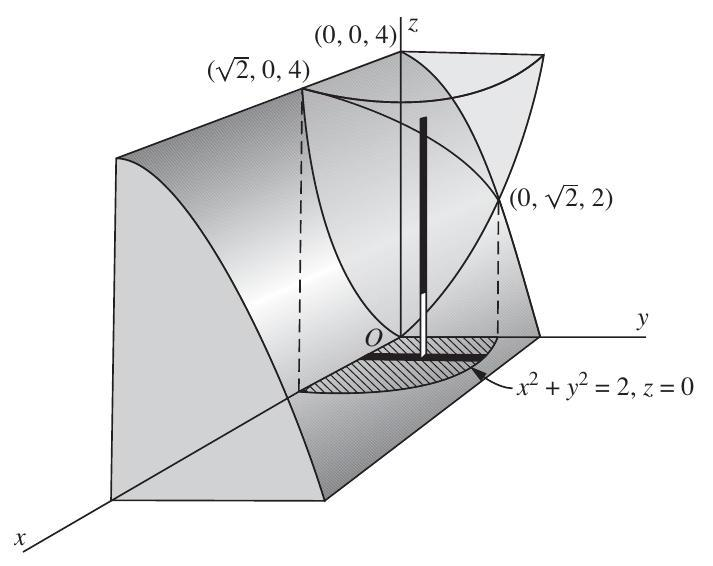
\includegraphics[max width=\textwidth]{2024_04_20_fe2e8e718cc0fcd63d1bg-05}
\end{center}

Fig. 57-6

\begin{enumerate}
  \setcounter{enumi}{6}
  \item Find the volume within the cylinder $r=4 \cos \theta$ bounded above by the sphere $r^{2}+z^{2}=16$ and below by the plane $z=0$. (See Fig. 57-7.)
\end{enumerate}

\begin{center}
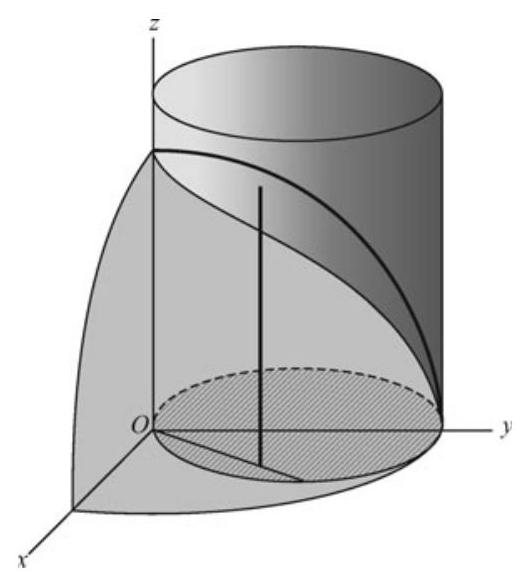
\includegraphics[max width=\textwidth]{2024_04_20_fe2e8e718cc0fcd63d1bg-05(1)}
\end{center}

Fig. 57-7

Integrate first with respect to $z$ from $z=0$ to $z=\sqrt{16-r^{2}}$, then with respect to $r$ from $r=0$ to $r=4 \cos \theta$, and finally with respect to $\theta$ from $\theta=0$ to $\theta=\pi$ to obtain the required volume. Thus,

$$
\begin{aligned}
V & =\int_{0}^{\pi} \int_{0}^{4 \cos \theta} \int_{0}^{\sqrt{16-r^{2}}} r d z d y d \theta=\int_{0}^{\pi} \int_{0}^{4 \cos \theta} r \sqrt{16-r^{2}} d r d \theta \\
& =-\frac{64}{3} \int_{0}^{\pi}\left(\sin ^{3} \theta-1\right) d \theta=\frac{64}{9}(3 \pi-4) \text { cubic units }
\end{aligned}
$$

\begin{enumerate}
  \setcounter{enumi}{7}
  \item Find the coordinates of the centroid of the volume within the cylinder $r=2 \cos \theta$, bounded above by the paraboloid $z=r^{2}$ and below by the plane $z=0$. (See Fig. 57-8.)
\end{enumerate}

$$
\begin{aligned}
V & =2 \int_{0}^{\pi / 2} \int_{0}^{2 \cos \theta} \int_{0}^{r^{2}} r d z d r d \theta=2 \int_{0}^{\pi / 2} \int_{0}^{2 \cos \theta} r^{2} d r d \theta \\
& =\frac{1}{2} \int_{0}^{\pi / 2}\left[r^{4}\right]_{0}^{2 \cos \theta} d \theta=8 \int_{0}^{\pi / 2} \cos ^{4} \theta d \theta=\frac{3}{2} \pi \\
M_{y z} & =\iiint_{R} x d V=2 \int_{0}^{\pi / 2} \int_{0}^{2 \cos \theta} \int_{0}^{r^{2}}(r \cos \theta) r d z d r d \theta \\
& =2 \int_{0}^{\pi / 2} \int_{0}^{2 \cos \theta} r^{4} \cos \theta d r d \theta=\frac{64}{5} \int_{0}^{\pi / 2} \cos ^{6} \theta d \theta=2 \pi
\end{aligned}
$$

\begin{center}
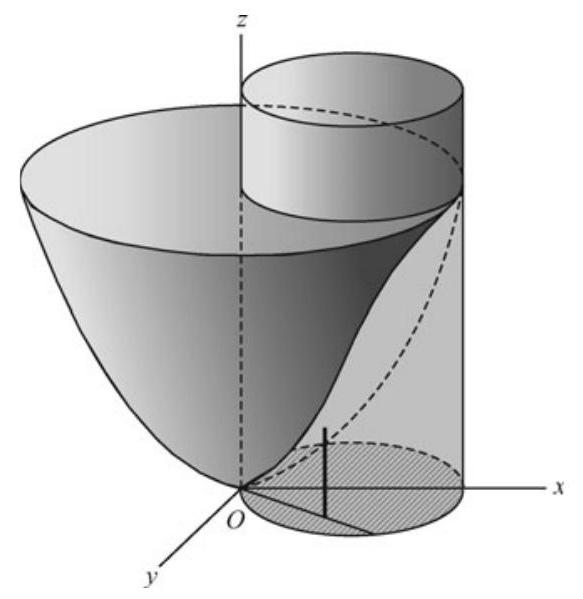
\includegraphics[max width=\textwidth]{2024_04_20_fe2e8e718cc0fcd63d1bg-06}
\end{center}

Fig. $57-8$

Then $\bar{x}=M_{y z} / V=\frac{4}{3}$. By symmetry, $\bar{y}=0$. Also,

$$
\begin{aligned}
M_{x y} & =\iiint_{R} z d V=2 \int_{0}^{\pi / 2} \int_{0}^{2 \cos \theta} \int_{0}^{r^{2}} z r d z d r d \theta=\int_{0}^{\pi / 2} \int_{0}^{2 \cos \theta} r^{5} d r d \theta \\
& =\frac{32}{3} \int_{0}^{\pi / 2} \cos ^{6} \theta d \theta=\frac{5}{3} \pi
\end{aligned}
$$

and $\bar{z}=M_{x y} / V=\frac{10}{9}$. Thus, the centroid has coordinates $\left(\frac{4}{3}, 0, \frac{10}{9}\right)$.

\begin{enumerate}
  \setcounter{enumi}{8}
  \item For the right circular cone of radius $a$ and height $h$, find (a) the centroid; (b) the moment of inertia with respect to its axis; (c) the moment of inertia with respect to any line through its vertex and perpendicular to its axis; (d) the moment of inertia with respect to any line through its centroid and perpendicular to its axis; and (e) the moment of inertia with respect to any diameter of its base.
\end{enumerate}

Take the cone as in Fig. 57-9, so that its equation is $r=\frac{a}{h} z$. Then:

$$
\begin{aligned}
V & =4 \int_{0}^{\pi / 2} \int_{0}^{a} \int_{h r / a}^{h} r d z d r d \theta=4 \int_{0}^{\pi / 2} \int_{0}^{a}\left(h r-\frac{h}{a} r^{2}\right) d r d \theta \\
& =\frac{2}{3} h a^{2} \int_{0}^{\pi / 2} d \theta=\frac{1}{3} \pi h a^{2}
\end{aligned}
$$

\begin{center}
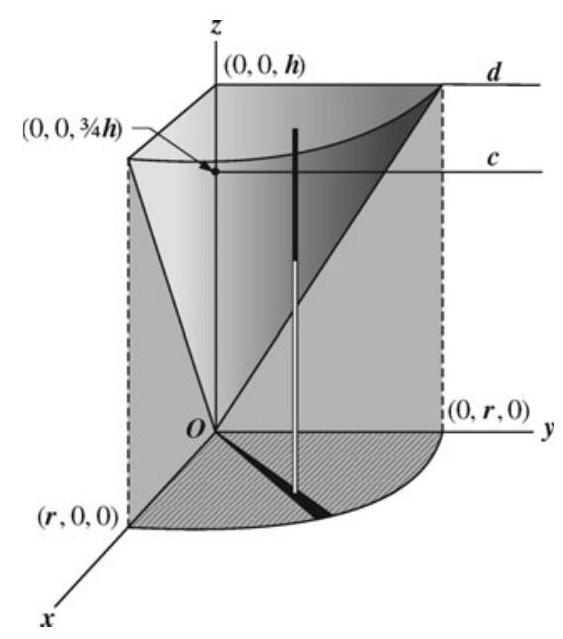
\includegraphics[max width=\textwidth]{2024_04_20_fe2e8e718cc0fcd63d1bg-06(1)}
\end{center}

Fig. $57-9$\\
(a) The centroid lies on the $z$ axis, and we have

$$
\begin{aligned}
M_{x y} & =\iiint_{R} z d V=4 \int_{0}^{\pi / 2} \int_{0}^{a} \int_{h r / a}^{h} z r d z d r d \theta \\
& =2 \int_{0}^{\pi / 2} \int_{0}^{a}\left(h^{2} r-\frac{h^{2}}{a^{2}} r^{3}\right) d r d \theta=\frac{1}{2} h^{2} a^{2} \int_{0}^{\pi / 2} d \theta=\frac{1}{4} \pi h^{2} a^{2}
\end{aligned}
$$

Then $\bar{z}=M_{x y} / V=\frac{3}{4} h$, and the centroid has coordinates $\left(0,0, \frac{3}{4} h\right)$.

(b) $I_{z}=\iiint_{R}\left(x^{2}+y^{2}\right) d V=4 \int_{0}^{\pi / 2} \int_{0}^{a} \int_{h r l a}^{h}\left(r^{2}\right) r d z d r d \theta=\frac{1}{10} \pi h a^{4}=\frac{3}{10} a^{2} V$

(c) Take the line as the $y$ axis. Then

$$
\begin{aligned}
I_{y} & =\iiint_{R}\left(x^{2}+z^{2}\right) d V=4 \int_{0}^{\pi / 2} \int_{0}^{a} \int_{h r / a}^{h}\left(r^{2} \cos ^{2} \theta+z^{2}\right) r d z d r d \theta \\
& =4 \int_{0}^{\pi / 2} \int_{0}^{a}\left[\left(h r^{3}-\frac{h}{a} r^{4}\right) \cos ^{2} \theta+\frac{1}{3}\left(h^{3} r-\frac{h^{3}}{a^{3}} r^{4}\right)\right] d r d \theta \\
& =\frac{1}{5} \pi h a^{2}\left(h^{2}+\frac{1}{4} a^{2}\right)=\frac{3}{5}\left(h^{2}+\frac{1}{4} a^{2}\right) V
\end{aligned}
$$

(d) Let the line $c$ through the centroid be parallel to the $y$ axis.

$$
I_{y}=I_{c}+V\left(\frac{3}{4} h\right)^{2} \quad \text { and } \quad I_{c}=\frac{3}{5}\left(h^{2}+\frac{1}{4} a^{2}\right) V-\frac{9}{16} h^{2} V=\frac{3}{80}\left(h^{2}+4 a^{2}\right) V
$$

(e) Let $d$ denote the diameter of the base of the cone parallel to the $y$ axis. Then

$$
I_{d}=I_{c}+V\left(\frac{1}{4} h\right)^{2}=\frac{3}{80}\left(h^{2}+4 a^{2}\right) V+\frac{1}{16} h^{2} V=\frac{1}{20}\left(2 h^{2}+3 a^{2}\right) V
$$

\begin{enumerate}
  \setcounter{enumi}{9}
  \item Find the volume cut from the cone $\phi=\frac{1}{4} \pi$ by the sphere $\rho=2 a \cos \phi$. (See Fig. 57-10.)
\end{enumerate}

$$
\begin{aligned}
V & =4 \iint_{R} d V=4 \int_{0}^{\pi / 2} \int_{0}^{\pi / 4} \int_{0}^{2 a \cos \phi} \rho^{2} \sin \phi d \rho d \phi d \theta \\
& =\frac{32 a^{3}}{3} \int_{0}^{\pi / 2} \int_{0}^{\pi / 4} \cos ^{3} \phi \sin \phi d \phi d \theta=2 a^{3} \int_{0}^{\pi / 2} d \theta=\pi a^{3} \text { cubic units }
\end{aligned}
$$

\begin{center}
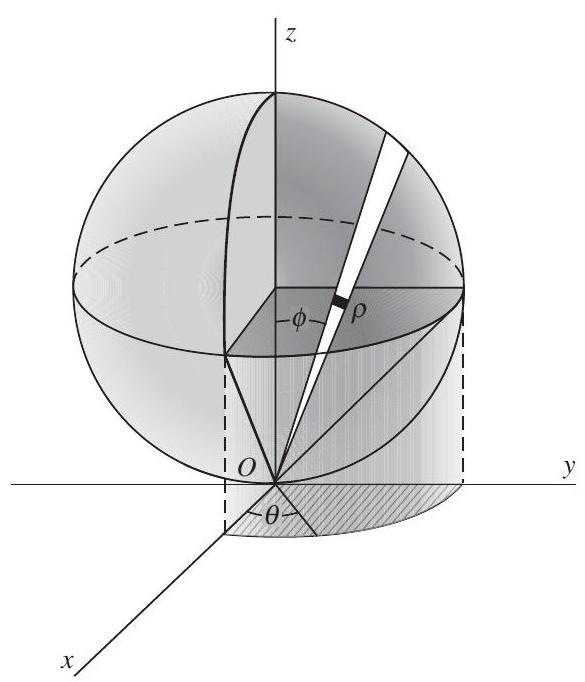
\includegraphics[max width=\textwidth]{2024_04_20_fe2e8e718cc0fcd63d1bg-07}
\end{center}

Fig. 57-10

\begin{enumerate}
  \setcounter{enumi}{10}
  \item Locate the centroid of the volume cut from one nappe of a cone of vertex angle $60^{\circ}$ by a sphere of radius 2 whose center is at the vertex of the cone.
\end{enumerate}

Take the surface as in Fig. 57-11, so that $x=y=0$. In spherical coordinates, the equation of the cone is $\phi=\pi / 6$, and the equation of the sphere is $\rho=2$. Then

$$
\begin{aligned}
V & =\iiint_{R} d V=4 \int_{0}^{\pi / 2} \int_{0}^{\pi / 6} \int_{0}^{2} \rho^{2} \sin \phi d \rho d \phi d \theta=\frac{32}{3} \int_{0}^{\pi / 2} \int_{0}^{\pi / 6} \sin \phi d \phi d \theta \\
& =-\frac{32}{3}\left(\frac{\sqrt{3}}{2}-1\right) \int_{0}^{\pi / 2} d \theta=\frac{8 \pi}{3}(2-\sqrt{3}) \\
M_{x y} & =\iiint_{R} z d V=4 \int_{0}^{\pi / 2} \int_{0}^{\pi / 6} \int_{0}^{2}(\rho \cos \phi) \rho^{2} \sin \phi d \rho d \phi d \theta \\
& =8 \int_{0}^{\pi / 2} \int_{0}^{\pi / 6} \sin 2 \phi d \phi d \theta=\pi
\end{aligned}
$$

and $\bar{z}=M_{x y} / V=\frac{3}{8}(2+\sqrt{3})$.

\begin{center}
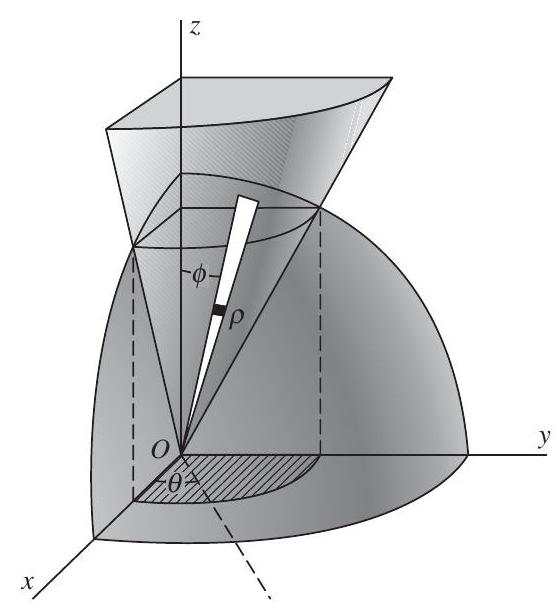
\includegraphics[max width=\textwidth]{2024_04_20_fe2e8e718cc0fcd63d1bg-08}
\end{center}

Fig. 57-11

\begin{enumerate}
  \setcounter{enumi}{11}
  \item Find the moment of inertia with respect to the $z$ axis of the volume of Problem 11.
\end{enumerate}

$$
\begin{aligned}
I_{z} & =\iiint_{R}\left(x^{2}+y^{2}\right) d V=4 \int_{0}^{\pi / 2} \int_{0}^{\pi / 6} \int_{0}^{2}\left(\rho^{2} \sin ^{2} \phi\right) \rho^{2} \sin \phi d \rho d \phi d \theta \\
& =\frac{128}{5} \int_{0}^{\pi / 2} \int_{0}^{\pi / 6} \sin ^{3} \phi d \phi d \theta=\frac{128}{5}\left(\frac{2}{3}-\frac{3}{8} \sqrt{3}\right) \int_{0}^{\pi / 2} d \theta=\frac{8 \pi}{15}(16-9 \sqrt{3})=\frac{5-2 \sqrt{3}}{5} V
\end{aligned}
$$

\section*{SUPPLEMENTARY PROBLEMS}
\begin{enumerate}
  \setcounter{enumi}{12}
  \item Describe the curve determined by each of the following pairs of equations in cylindrical coordinates:
\end{enumerate}

(a) $r=1, z=2$; (b) $r=2, z=\theta$; (c) $\theta=\pi / 4, r=\sqrt{2}$; (d) $\theta=\pi / 4, z=r$.

Ans. (a) circle of radius 1 in plane $z=2$ with center having rectangular coordinates $(0,0,2)$; (b) helix on right circular cylinder $r=2$; (c) vertical line through point having rectangular coordinates (1,1,0); (d) line through origin in plane $\theta=\pi / 4$, making an angle of $45^{\circ}$ with $x y$ plane

\begin{enumerate}
  \setcounter{enumi}{13}
  \item Describe the curve determined by each of the following pairs of equations in spherical coordinates:
\end{enumerate}

(a) $\rho=1, \theta=\pi$; (b) $\theta=\frac{\pi}{4}, \phi=\frac{\pi}{6}$; (c) $\rho=2, \phi=\frac{\pi}{4}$.

Ans. (a) circle of radius 1 in $x z$ plane with center at origin; (b) halfline on intersection of plane $\theta=\pi / 4$ and cone $\phi=\pi / 6$; (c) circle of radius $\sqrt{2}$ in plane $z=\sqrt{2}$ with center on $z$ axis

\begin{enumerate}
  \setcounter{enumi}{14}
  \item Transform each of the following equations in either rectangular, cylindrical, or spherical coordinates into equivalent equations in the two other coordinate systems:
\end{enumerate}

(a) $\rho=5$; (b) $z^{2}=r^{2}$; (c) $x^{2}+y^{2}+(z-1)^{2}=1$

Ans. (a) $x^{2}+y^{2}+z^{2}=25, r^{2}+z^{2}=25$; (b) $z^{2}=x^{2}+y^{2}, \cos ^{2} \phi=\frac{1}{2}$ (that is, $\phi=\pi / 4$ or $\phi=3 \pi / 4$ ); (c) $r^{2}+z^{2}=2 z$, $\rho=2 \cos \phi$

\begin{enumerate}
  \setcounter{enumi}{15}
  \item Evaluate the triple integral on the left in each of the following:
\end{enumerate}

(a) $\int_{0}^{1} \int_{1}^{2} \int_{2}^{3} d z d x d y=1$

(b) $\int_{0}^{1} \int_{x^{2}}^{x} \int_{0}^{x y} d z d y d x=\frac{1}{24}$

(c) $\int_{0}^{6} \int_{0}^{12-2 y} \int_{0}^{4-2 y / 3-x / 3} x d z d x d y=144 \quad\left[=\int_{0}^{12} \int_{0}^{6-x / 2} \int_{0}^{4-2 y / 3-x / 3} x d z d y d x\right]$

(d) $\int_{0}^{\pi / 2} \int_{0}^{4} \int_{0}^{\sqrt{16-z^{2}}}\left(16-r^{2}\right)^{1 / 2} r z d r d \theta=\frac{256}{5} \pi$

(e) $\int_{0}^{2 \pi} \int_{0}^{\pi} \int_{0}^{5} \rho^{4} \sin \phi d \rho d \phi d \theta=2500 \pi$

\begin{enumerate}
  \setcounter{enumi}{16}
  \item Evaluate the integral of Problem 16(b) after changing the order to $d z d x d y$.

  \item Evalute the integral of Problem 16(c), changing the order to $d x d y d z$ and to $d y d z d x$.

  \item Find the following volumes, using integrals in rectangular coordinates:\\
(a) Inside $x^{2}+y^{2}=9$, above $z=0$, and below $x+z=4$\\
Ans. $36 \pi$ cubic units\\
(b) Bounded by the coordinate planes and $6 x+4 y+3 z=12$\\
Ans. 4 cubic units\\
(c) Inside $x^{2}+y^{2}=4 x$, above $z=0$, and below $x^{2}+y^{2}=4 z$\\
Ans. $6 \pi$ cubic units

  \item Find the following volumes, using triple integrals in cylindrical coordinates:

\end{enumerate}

(a) The volume of Problem 4.

(b) The volume of Problem 19(c).

(c) That inside $r^{2}=16$, above $z=0$, and below $2 z=y$

Ans. $64 / 3$ cubic units

\begin{enumerate}
  \setcounter{enumi}{20}
  \item Find the centroid of each of the following volumes:
\end{enumerate}

(a) Under $z^{2}=x y$ and above the triangle $y=x, y=0$,

$x=4$ in the plane $z=0$

(b) That of Problem 19(b)

(c) The first-octant volume of Problem 19(a)

(d) That of Problem 19(c)

(e) That of Problem 20(c)\\
Ans. $\left(3, \frac{9}{5}, \frac{9}{8}\right)$

Ans. $\left(\frac{1}{2}, \frac{3}{4}, 1\right)$

Ans. $\left(\frac{64-9 \pi}{16(\pi-1)}, \frac{23}{8(\pi-1)}, \frac{73 \pi-128}{32(\pi-1)}\right)$

Ans. $\left(\frac{8}{3}, 0, \frac{10}{9}\right)$

Ans. $(0,3 \pi / 4,3 \pi / 16)$

\begin{enumerate}
  \setcounter{enumi}{21}
  \item Find the moments of inertia $I_{x}, I_{y}, I_{z}$ of the following volumes:
\end{enumerate}

(a) That of Problem 4

(b) That of Problem 19(b)

(c) That of Problem 19(c)

(d) That cut from $z=r^{2}$ by the plane $z=2$

$$
\begin{array}{ll}
\text { Ans. } & I_{x}=I_{y}=\frac{32}{3} V ; I_{z}=\frac{16}{3} V \\
\text { Ans. } & I_{x}=\frac{5}{2} V ; I_{y}=2 V ; I_{z}=\frac{13}{10} V \\
\text { Ans. } & I_{x}=\frac{55}{18} V ; I_{y}=\frac{175}{18} V ; I_{z}=\frac{80}{9} V \\
\text { Ans. } & I_{x}=I_{y}=\frac{7}{3} V ; I_{z}=\frac{2}{3} V
\end{array}
$$

\begin{enumerate}
  \setcounter{enumi}{22}
  \item Show that, in cylindrical coordinates, the triple integral of a function $f(r, \theta, z)$ over a region $R$ may be represented by
\end{enumerate}

$$
\int_{\alpha}^{\beta} \int_{r_{1}(\theta)}^{r_{2}(\theta)} \int_{z_{1}(r, \theta)}^{z_{2}(r, \theta)} f(r, \theta, z) r d z d r d \theta
$$

[Hint: Consider, in Fig. 57-12, a representative subregion of $R$ bounded by two cylinders having the $z$ axis as axis and of radii $r$ and $r+\Delta r$, respectively, cut by two horizontal planes through $(0,0, z)$ and $(0,0, z+\Delta z)$, respectively, and by two vertical planes through the $z$ axis making angles $\theta$ and $\theta+\Delta \theta$, respectively, with the $x z$ plane. Take $\Delta V=(r \Delta \theta) \Delta r \Delta z$ as an approximation of its volume.]

\begin{center}
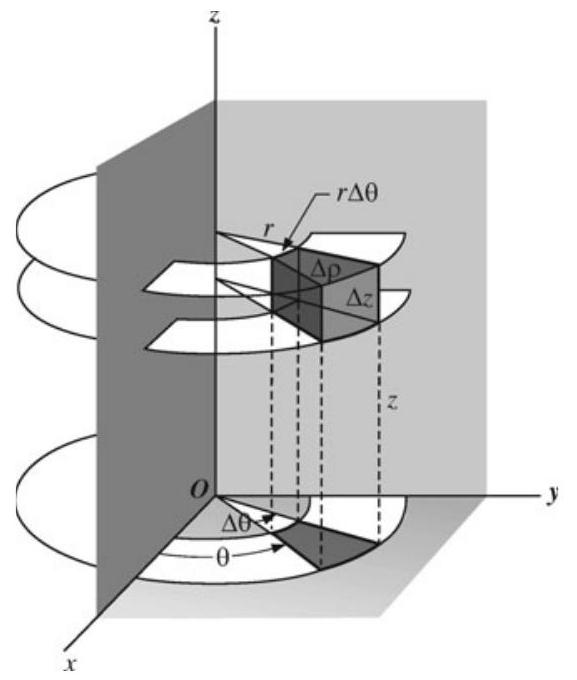
\includegraphics[max width=\textwidth]{2024_04_20_fe2e8e718cc0fcd63d1bg-10}
\end{center}

Fig. 57-12

\begin{enumerate}
  \setcounter{enumi}{23}
  \item Show that, in spherical coordinates, the triple integral of a function $f(\rho, \phi, \theta)$ over a region $R$ may be represented by
\end{enumerate}

$$
\int_{\alpha}^{\beta} \int_{\phi_{1}(\theta)}^{\phi_{2}(\theta)} \int_{\rho_{1}(\phi, \theta)}^{\rho_{2}(\phi, \theta)} f(\rho, \phi, \theta) \rho^{2} \sin \phi d \rho d \phi d \theta
$$

[Hint: Consider, in Fig. 57-13, a representative subregion of $R$ bounded by two spheres centered at $O$, of radii $\rho$ and $\rho+\Delta \rho$, respectively, by two cones having $O$ as vertex, the $z$ axis as axis, and semivertical angles $\phi$ and $\phi+\Delta \phi$, respectively, and by two vertical planes through the $z$ axis making angles $\theta$ and $\theta+\Delta \theta$, respectively, with the $y z$ plane. Take $\Delta V=(\rho \Delta \phi)(\rho \sin \phi \Delta \theta)(\Delta \rho)=\rho^{2} \sin \phi \Delta \rho \Delta \phi \Delta \theta$ as an approximation of its volume.]

\begin{enumerate}
  \setcounter{enumi}{24}
  \item Change the following points from rectangular to cylindrical coordinates: (a) $(1,0,0)$; (b) $(\sqrt{2}, \sqrt{2}, 2)$;
\end{enumerate}

(c) $(-\sqrt{3}, 1,5)$.

Ans.

(a) $(1,0,0) ;$ (b) $\left(2, \frac{\pi}{4}, 1\right) ;$ (c) $\left(2, \frac{5 \pi}{6}, 5\right)$

\begin{center}
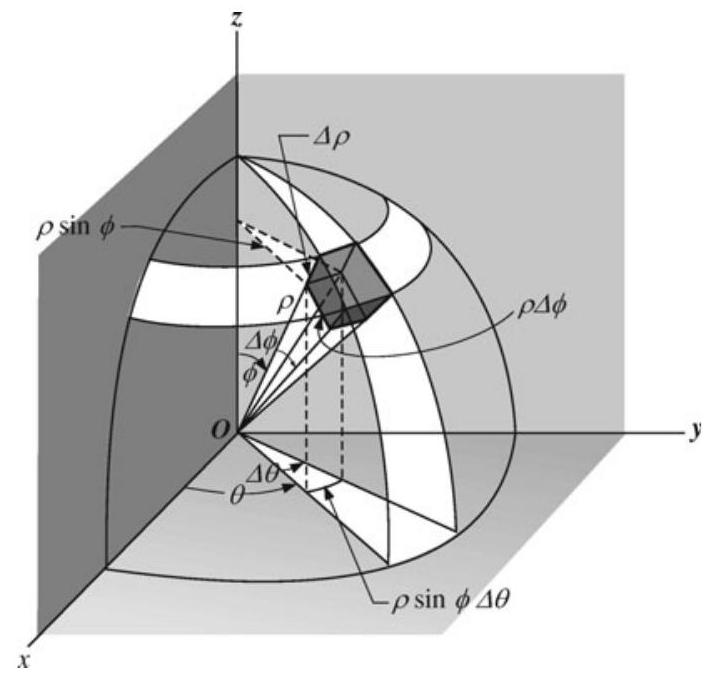
\includegraphics[max width=\textwidth]{2024_04_20_fe2e8e718cc0fcd63d1bg-11}
\end{center}

Fig. 57-13

\begin{enumerate}
  \setcounter{enumi}{25}
  \item Change the following points from cylindrical to rectangular coordinates: (a) $\left(5, \frac{\pi}{3}, 1\right)$; (b) $\left(2,-\frac{\pi}{6}, 0\right)$; (c) $(0,7,1)$. Ans.
\end{enumerate}

$$
\text { (a) }\left(\frac{5}{2}, \frac{5 \sqrt{3}}{2}, 1\right) ;(b)(\sqrt{3},-1,0) ; \text { (c) }(0,0,1)
$$

\begin{enumerate}
  \setcounter{enumi}{26}
  \item Change the following points from rectangular to spherical coordinates: (a) $(1,0,0)$; (b) $(\sqrt{2}, \sqrt{2}, 2)$;
\end{enumerate}

(c) $(1,-1,-\sqrt{2})$.

Ans. (a) $\left(1,0, \frac{\pi}{2}\right)$; (b) $\left(2 \sqrt{2}, \frac{\pi}{4}, \frac{\pi}{4}\right) ;$ (c) $\left(2, \frac{7 \pi}{4}, \frac{3 \pi}{4}\right)$

\begin{enumerate}
  \setcounter{enumi}{27}
  \item Change the following points from spherical to rectangular coordinates: (a) $(1,0,0)$; (b) $(2,0, \pi)$; (c) $\left(4, \frac{\pi}{4}, \frac{\pi}{6}\right)$. Ans. (a) $(0,0,1)$; (b) $(0,0,-2)$; (c) $(\sqrt{2}, \sqrt{2}, 2 \sqrt{3})$

  \item Describe the surfaces determined by the following equations:\\
(a) $z=r^{2}$; (b) $r=4 \cos \theta$; (c) $\rho \cos \phi=4$;\\
(d) $\rho \sin \phi=4$;\\
(e) $\phi=\frac{\pi}{2}$; (f) $\theta=\frac{\pi}{4}$; (g) $\rho=2 \sin \phi$

\end{enumerate}

Ans. (a) circular paraboloid; (b) right circular cylinder $(x-2)^{2}+y^{2}=4$; (c) plane $z=4$; (d) right circular cylinder $x^{2}+y^{2}=16$; (e) the $x y$ plane; (f) right circular cone with the $z$ axis as its axis; (g) right circular cylinder $x^{2}+y^{2}=4$

\section*{CHAPTER 58}
\section*{Masses of Variable Density}
Homogeneous masses can be treated as geometric figures with density $\delta=1$. The mass of a homogeneous body of volume $V$ and density $\delta$ is $m=\delta V$.

For a nonhomogenous mass whose density $\delta$ varies continuously, an element of mass $d m$ is given by

(1) $\delta(x, y) d s$ for a planar material curve (e.g., a piece of fine wire);

(2) $\delta(x, y) d A$ for a material two-dimensional plate (e.g., a thin sheet of metal);

(3) $\delta(x, y, z) d V$ for a material body.

The center of mass $(\bar{x}, \bar{y})$ of a planar plate that is distributed over a region $R$ with density $\delta(x, y)$ is determined by the equations

$$
m \bar{x}=M_{y} \quad \text { and } \quad m \bar{y}=M_{x}, \quad \text { where } \quad M_{y}=\iint_{R} \delta(x, y) x d A \quad \text { and } \quad M_{x}=\iint_{R} \delta(x, y) y d A
$$

An analogous result holds for the center of mass of a three-dimensional body. The reasoning is similar to that for centroids in Chapter 55.

The moments of inertia of a planar mass with respect to the $x$ axis and the $y$ axis are $I_{x}=\iint_{R} \delta(x, y) y^{2} d A$ and $I_{y}=\iint_{R} \delta(x, y) x^{2} d A$. Similar formulas with triple integrals hold for three-dimensional bodies. (For example, $I_{x}=\iiint_{R} \delta(x, y, z)\left(y^{2}+z^{2}\right) d A$.)

\section*{SOLVED PROBLEMS}
\begin{enumerate}
  \item Find the mass of a semicircular wire whose density varies as the distance from the diameter joining the ends.
\end{enumerate}

Take the wire as in Fig. 58-1, so that $\delta(x, y)=k y$. Then, from $x^{2}+y^{2}=r^{2}$.

and

$$
\begin{aligned}
d s & =\sqrt{1+\left(\frac{d y}{d x}\right)^{2}} d x=\frac{r}{y} d x \\
m & =\int \delta(x, y) d s=\int_{-r}^{r} k y \frac{r}{y} d x=k r \int_{-r}^{r} d x=2 k r^{2} \text { units }
\end{aligned}
$$

\begin{center}
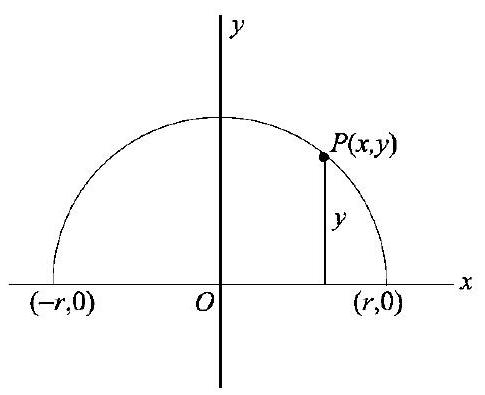
\includegraphics[max width=\textwidth]{2024_04_20_fe2e8e718cc0fcd63d1bg-12}
\end{center}

Fig. 58-1

\begin{enumerate}
  \setcounter{enumi}{1}
  \item Find the mass of a square plate of side $a$ if the density varies as the square of the distance from a vertex.
\end{enumerate}

Take the square as in Fig. 58-2, and let the vertex from which distances are measured be at the origin. Then $\delta(x, y)=k\left(x^{2}+y^{2}\right)$ and

$$
m=\iint_{R} \delta(x, y) d A=\int_{0}^{a} \int_{0}^{a} k\left(x^{2}+y^{2}\right) d x d y=k \int_{0}^{a}\left(\frac{1}{3} a^{3}+a y^{2}\right) d y=\frac{2}{3} k a^{4} \text { units }
$$

\begin{center}
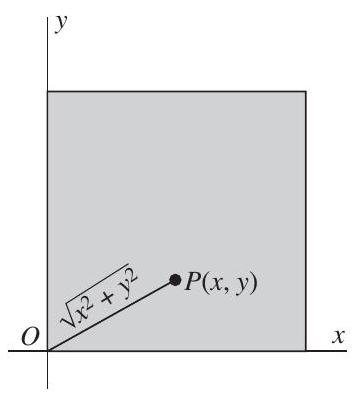
\includegraphics[max width=\textwidth]{2024_04_20_fe2e8e718cc0fcd63d1bg-13(1)}
\end{center}

Fig. $58-2$

\begin{enumerate}
  \setcounter{enumi}{2}
  \item Find the mass of a circular plate of radius $r$ if the density varies as the square of the distance from a point on the circumference.
\end{enumerate}

Take the circle as in Fig. 58-3 and let $A(r, 0)$ be the fixed point on the circumference. Then $\delta(x, y)=$ $k\left[(x-r)^{2}+y^{2}\right]$ and

$$
m=\iint_{R} \delta(x, y) d A=2 \int_{-r}^{r} \int_{0}^{\sqrt{r^{2}-x^{2}}} k\left[(x-r)^{2}+y^{2}\right] d y d x=\frac{3}{2} k \pi r^{4} \text { units }
$$

\begin{center}
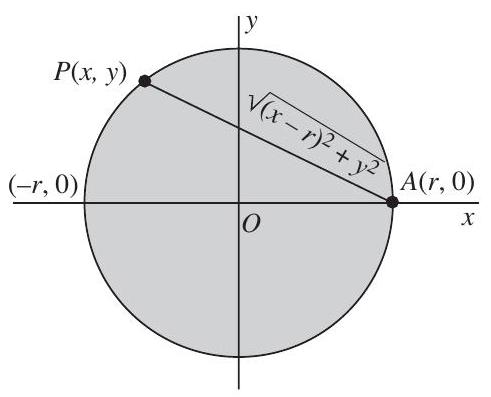
\includegraphics[max width=\textwidth]{2024_04_20_fe2e8e718cc0fcd63d1bg-13}
\end{center}

Fig. 58-3

\begin{enumerate}
  \setcounter{enumi}{3}
  \item Find the center of mass of a plate in the form of the segments cut from the parabola $y^{2}=8 x$ by its latus rectum $x=2$ if the density varies as the distance from the latus rectum. (See Fig. 58-4.)
\end{enumerate}

Here, $\delta(x, y)=2-x$ and, by symmetry, $\bar{y}=0$. For the upper half of the plate,

$$
\begin{aligned}
m & =\iint_{R} \delta(x, y) d A=\int_{0}^{4} \int_{y^{2} / 8}^{2} k(2-x) d x d y=k \int_{0}^{4}\left(2-\frac{y^{2}}{4}+\frac{y^{4}}{128}\right) d y=\frac{64}{15} k \\
M_{y} & =\iint_{R} \delta(x, y) x d A=\int_{0}^{4} \int_{y^{2} / 8}^{2} k(2-x) x d x d y=k \int_{0}^{4}\left[\frac{4}{3}-\frac{y^{4}}{64}+\frac{y^{6}}{(24)(64)}\right] d y=\frac{128}{35} k
\end{aligned}
$$

and $\bar{x}=M_{y} / m=\frac{6}{7}$. The center of mass has coordinates $\left(\frac{6}{7}, 0\right)$.

\begin{center}
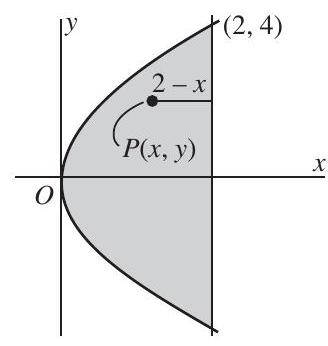
\includegraphics[max width=\textwidth]{2024_04_20_fe2e8e718cc0fcd63d1bg-14}
\end{center}

Fig. 58-4

\begin{enumerate}
  \setcounter{enumi}{4}
  \item Find the center of mass of a plate in the form of the upper half of the cardioid $r=2(1+\cos \theta)$ if the density varies as the distance from the pole. (See Fig. 58-5.)
\end{enumerate}

$$
\begin{aligned}
m & =\iint_{R} \delta(r, \theta) d A=\int_{0}^{\pi} \int_{0}^{2(1+\cos \theta)}(k r) r d r d \theta=\frac{8}{3} k \int_{0}^{\pi}(1+\cos \theta)^{3} d \theta=\frac{20}{3} k \pi \\
M_{x} & =\iint_{R} \delta(r, \theta) y d A=\int_{0}^{\pi} \int_{0}^{2(1+\cos \theta)}(k r)(r \sin \theta) r d r d \theta \\
& =4 k \int_{0}^{\pi}(1+\cos \theta)^{4} \sin \theta d \theta=\frac{128}{5} k \\
M_{y} & =\iint_{R} \delta(r, \theta) x d A=\int_{0}^{\pi} \int_{0}^{2(1+\cos \theta)}(k r)(r \cos \theta) r d r d \theta=14 k \pi
\end{aligned}
$$

Then $\bar{x}=\frac{M_{y}}{m}=\frac{21}{10}, \bar{y}=\frac{M_{x}}{m}=\frac{96}{25 \pi}$, and the center of mass has coordinates $\left(\frac{21}{10}, \frac{96}{25 \pi}\right)$.

\begin{center}
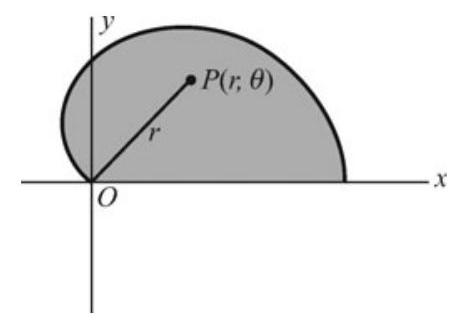
\includegraphics[max width=\textwidth]{2024_04_20_fe2e8e718cc0fcd63d1bg-14(1)}
\end{center}

Fig. 58-5

\begin{enumerate}
  \setcounter{enumi}{5}
  \item Find the moment of inertia with respect to the $x$ axis of the plate having for edges one arch of the curve $y=\sin x$ and the $x$ axis if its density varies as the distance from the $x$ axis. (See Fig. 58-6.)
\end{enumerate}

$$
\begin{aligned}
& m=\iint_{R} \delta(x, y) d A=\int_{0}^{\pi} \int_{0}^{\sin x} k y d y d x=\frac{1}{2} k \int_{0}^{\pi} \sin ^{2} x d x=\frac{1}{4} k \pi \\
& I_{x}=\iint_{R} \delta(x, y) y^{2} d A=\int_{0}^{\pi} \int_{0}^{\sin x}(k y)\left(y^{2}\right) d y d x=\frac{1}{4} k \int_{0}^{\pi} \sin ^{4} x d x=\frac{3}{32} k \pi=\frac{3}{8} m
\end{aligned}
$$

\begin{center}
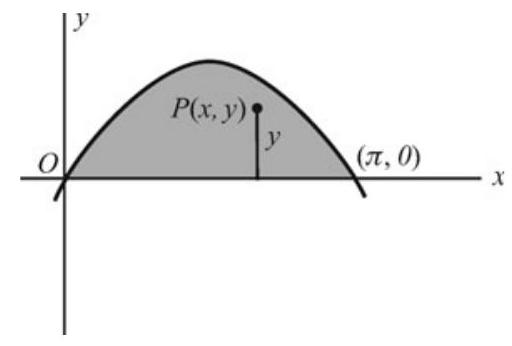
\includegraphics[max width=\textwidth]{2024_04_20_fe2e8e718cc0fcd63d1bg-14(2)}
\end{center}

Fig. 58-6

\begin{enumerate}
  \setcounter{enumi}{6}
  \item Find the mass of a sphere of radius $a$ if the density varies inversely as the square of the distance from the center. Take the sphere as in Fig. 58-7. Then $\delta(x, y, z)=\frac{k}{x^{2}+y^{2}+z^{2}}=\frac{k}{\rho^{2}}$ and
\end{enumerate}

$$
\begin{aligned}
m & =\iiint_{R} \delta(x, y, z) d V=8 \int_{0}^{\pi / 2} \int_{0}^{\pi / 2} \int_{0}^{a} \frac{k}{\rho^{2}} \rho^{2} \sin \phi d \rho d \phi d \theta \\
& =8 k a \int_{0}^{\pi / 2} \int_{0}^{\pi / 2} \sin \phi d \phi d \theta=8 k a \int_{0}^{\pi / 2} d \theta=4 k \pi a \text { units }
\end{aligned}
$$

\begin{center}
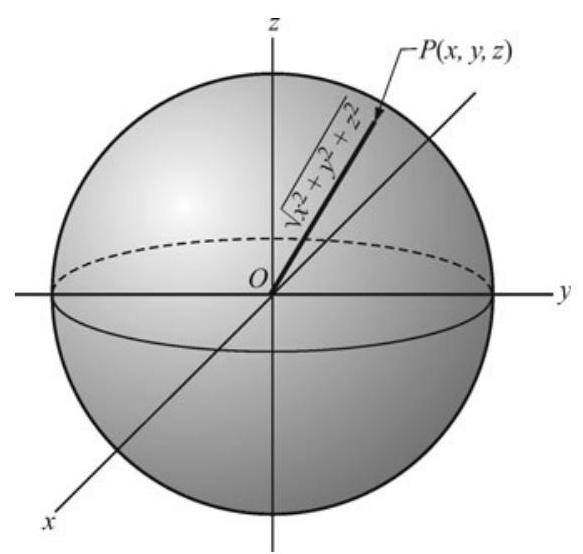
\includegraphics[max width=\textwidth]{2024_04_20_fe2e8e718cc0fcd63d1bg-15}
\end{center}

Fig. 58-7

\begin{enumerate}
  \setcounter{enumi}{7}
  \item Find the center of mass of a right circular cylinder of radius $a$ and height $h$ if the density varies as the distance from the base.
\end{enumerate}

Take the cylinder as in Fig. 58-8, so that its equation is $r=a$ and the volume in question is that part of the cylinder between the planes $z=0$ and $z=h$. Clearly, the center of mass lies on the $z$ axis. Then

$$
\begin{aligned}
m & =\iiint_{R} \delta(z, r, \theta) d V=4 \int_{0}^{\pi / 2} \int_{0}^{a} \int_{0}^{h}(k z) r d z d r d \theta=2 k h^{2} \int_{0}^{\pi / 2} \int_{0}^{a} r d r d \theta \\
& =k h^{2} a^{2} \int_{0}^{\pi / 2} d \theta=\frac{1}{2} k \pi h^{2} a^{2} \\
M_{x y} & =\iiint_{R} \delta(z, r, \theta) z d V=4 \int_{0}^{\pi / 2} \int_{0}^{a} \int_{0}^{h}\left(k z^{2}\right) r d z d r d \theta=\frac{4}{3} k h^{3} \int_{0}^{\pi / 2} \int_{0}^{a} r d r d \theta \\
& =\frac{2}{3} k h^{3} a^{2} \int_{0}^{\pi / 2} d \theta=\frac{1}{3} k \pi h^{3} a^{2}
\end{aligned}
$$

and $\bar{z}=M_{x y} / m=\frac{2}{3} h$. Thus the center of mass has coordinates $\left(0,0, \frac{2}{3} h\right)$.

\begin{center}
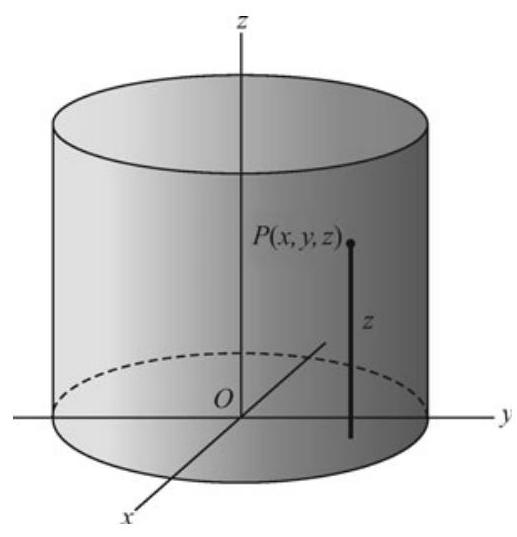
\includegraphics[max width=\textwidth]{2024_04_20_fe2e8e718cc0fcd63d1bg-15(1)}
\end{center}

Fig. 58-8

\section*{SUPPLEMENTARY PROBLEMS}
\begin{enumerate}
  \setcounter{enumi}{8}
  \item Find the mass of
\end{enumerate}

(a) A straight rod of length $a$ whose density varies as the square of the distance from one end

Ans. $\quad \frac{1}{3} k a^{3}$ units

(b) A plate in the form of a right triangle with legs $a$ and $b$, if the density varies as the sum of the distance from the legs

Ans. $\frac{1}{6} k a b(a+b)$ units

(c) A circular plate of radius $a$ whose density varies as the distance from the center

Ans. $\quad \frac{2}{3} k a^{3} \pi$ units

(d) A plate in the form of an ellipse $b^{2} x^{2}+a^{2} y^{2}=a^{2} b^{2}$, if the density varies as the sum of the distances from its axes

Ans. $\quad \frac{4}{3} k a b(a+b)$ units

(e) A circular cylinder of height $b$ and radius of base $a$, if the density varies as the square of the distance from its axis

Ans. $\quad \frac{1}{2} k a^{4} b \pi$ units

(f) A sphere of radius $a$ whose density varies as the distance from a fixed diametral plane

Ans. $\quad \frac{1}{2} k a^{4} \pi$ units

(g) $A$ circular cone of height $b$ and radius of base $a$ whose density varies as the distance from its axis

Ans. $\quad \frac{1}{6} k a^{3} b \pi$ units

(h) A spherical surface whose density varies as the distance from a fixed diametral plane

Ans. $2 k a^{3} \pi$ units

\begin{enumerate}
  \setcounter{enumi}{9}
  \item Find the center of mass of
\end{enumerate}

(a) One quadrant of the plate of Problem 9(c)

Ans. $(3 a / 2 \pi, 3 a / 2 \pi)$

(b) One quadrant of a circular plate of radius $a$, if the density varies as the distance from a bounding radius (the $x$ axis)

Ans. $(3 a / 8,3 a \pi / 16)$

(c) A cube of edge $a$, if the density varies as the sum of the distances from three adjacent edges (on the coordinate axes)

Ans. $(5 a / 9,5 a / 9,5 a / 9)$\\
(d) An octant of a sphere of radius $a$, if the density varies as the distance from one of the plane faces

Ans. $(16 a / 15 \pi, 16 a / 15 \pi, 8 a / 15)$

(e) A right circular cone of height $b$ and radius of base $a$, if the density varies as the distance from its base Ans. $\quad(0,0,2 b / 5)$

\begin{enumerate}
  \setcounter{enumi}{10}
  \item Find the moment of inertia of:
\end{enumerate}

(a) A square plate of side $a$ with respect to a side, if the density varies as the square of the distance from an extremity of that side

Ans. $\quad \frac{7}{15} a^{2} m$

(b) A plate in the form of a circle of radius $a$ with respect to its center, if the density varies as the square of the distance from the center

Ans. $\quad \frac{2}{3} a^{2} m$

(c) A cube of edge $a$ with respect to an edge, if the density varies as the square of the distance from one extremity of that edge

Ans. $\quad \frac{38}{45} a^{2} m$

(d) A right circular cone of height $b$ and radius of base $a$ with respect to its axis, if the density varies as the distance from the axis

Ans. $\quad \frac{2}{5} a^{2} m$

(e) The cone of (d), if the density varies as the distance from the base

Ans. $\quad \frac{1}{5} a^{2} m$

\section*{CHAPTER 59}
\section*{Differential Equations of First and Second Order}
A differential equation is an equation that involves a function, say $y$, of one variable, say $x$, and derivatives of $y$ or differentials of $x$ and $y$. Examples are $\frac{d^{2} y}{d x^{2}}+2 \frac{d y}{d x}+3 y-7 \sin x+4 x=0$ and $d y=(x+2 y) d x$. The first equation also can be written as $y^{\prime \prime}+2 y^{\prime}+3 y-7 \sin x+4 x=0$.

The order of a differential equation is the order of the derivative of highest order appearing in it. The first of the above equations is of order two, and the second is of order one.

A solution of a differential equation is a function $y$ that satisfies the equation. A general solution of an equation is a formula that describes all solutions of the equation. It turns out that a general solution of a differential equation of order $n$ will contain $n$ arbitrary constants.

\section*{Separable Differential Equations}
A separable differential equation is a first-order equation that can be put in the form

$$
f(x) d x+g(y) d y=0, \quad \text { which is equivalent to } \frac{d y}{d x}=-\frac{f(x)}{g(y)}
$$

A separable equation can be solved by taking antiderivatives

$$
\int f(x) d x+\int g(y) d y=C
$$

The result is an equation involving $x$ and $y$ that determines $y$ as a function of $x$. (See Problems 4-6, and for justification, see Problem 61.)

\section*{Homogeneous Functions}
A function $f(x, y)$ is said to be homogeneous of degree $n$ if $f(\lambda x, \lambda y)=\lambda^{n} f(x, y)$. The equation $M(x, y) d x+$ $N(x, y) d y=0$ is said to be homogeneous if $M(x, y)$ and $N(x, y)$ are homogeneous of the same degree. It is easy to verify that the substitution

$$
y=v x, \quad d y=v d x+x d v
$$

will transform a homogeneous equation into a separable equation in the variables $x$ and $v$.

\section*{Integrating Factors}
Certain differential equations may be solved after multiplication by a suitable function of $x$ and $y$ produces an integrable combination of terms. Such a function is called an integrating factor of the equations. In looking for integrable combinations, note that:\\
(i) $d(x y)=x d y+y d x$\\
(iii) $d(\ln x y)=\frac{x d y+y d x}{x y}$\\
(ii) $d(y / x)=\frac{x d y-y d x}{x^{2}}$\\
(iv) $d\left(\frac{1}{k+1} u^{k+1}\right)=u^{k} d u$

Moreover, $d(F)+d(G)+\cdots=0$ yields $F+G+.=$ constant. (See Problems 10-14.)

The so-called linear differential equations of the first order, $\frac{d y}{d x}+P y=Q$, where $P$ and $Q$ are functions of $x$ alone, have the function $\xi(x)=e^{\int p d x}$ as integrating factor. (See Problems 15-17.)

An equation of the form $\frac{d y}{d x}+P y=Q y^{n}$, where $n \neq 0,1$ and where $P$ and $Q$ are functions of $x$ alone, can be reduced to the linear form by the substitution

$$
y^{1-n}=z, \quad y^{-n} \frac{d y}{d x}=\frac{1}{1-n} \frac{d z}{d x}
$$

(See Problems 18-19).

\section*{Second-Order Equations}
The second-order equations that will be solved in this chapter are of the following types:

\begin{center}
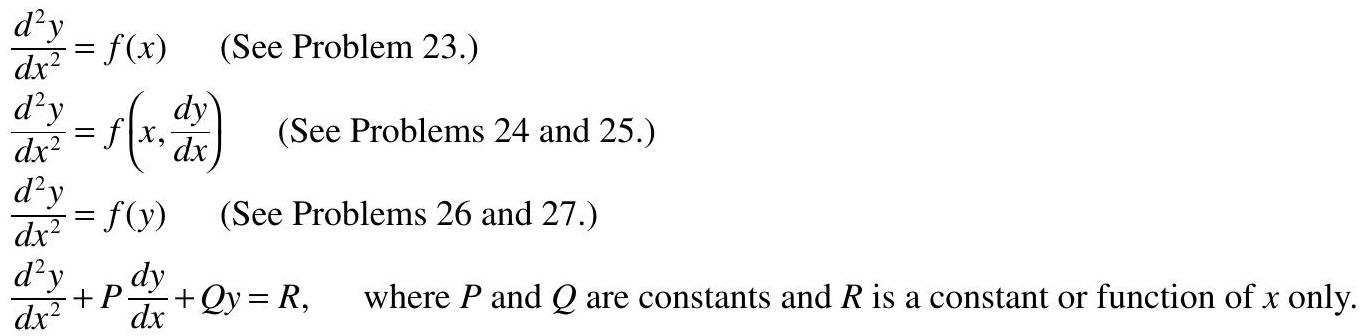
\includegraphics[max width=\textwidth]{2024_04_20_fe2e8e718cc0fcd63d1bg-19}
\end{center}

If the equation $m^{2}+P m+Q=0$ has two distinct roots $m_{1}$ and $m_{2}$, then $y=C_{1} e^{m_{1} x}+C_{2} e^{m_{2} x}$ is the general solution of the equation $\frac{d^{2} y}{d x^{2}}+P \frac{d y}{d x}+Q y=0$. If the two roots are identical so that $m_{1}=m_{2}=m$, then

$$
y=C_{1} e^{m x}+C_{2} x e^{m x}=e^{m x}\left(C_{1}+C_{2} x\right)
$$

is the general solution.

The general solution of $\frac{d^{2} y}{d x^{2}}+P \frac{d y}{d x}+Q y=0$ is called the complementary function of the equation


\begin{equation*}
\frac{d^{2} y}{d x^{2}}+P \frac{d y}{d x}+Q y=R(x) \tag{59.1}
\end{equation*}


If $f(x)$ satisfies (59.1), then the general solution of (59.1) is

$$
y=\text { complementary function }+f(x)
$$

The function $f(x)$ is called a particular solution of (59.1).

\section*{SOLVED PROBLEMS}
\begin{enumerate}
  \item Show that (a) $y=2 e^{x}$, (b) $y=3 x$, and (c) $y=C_{1} e^{x}+C_{2} x$, where $C_{1}$ and $C_{2}$ are arbitrary constants, are solutions of the differential equation $y^{\prime \prime}(1-x)+y^{\prime} x-y=0$
\end{enumerate}

(a) Differentiate $y=2 e^{x}$ twice to obtain $y^{\prime}=2 e^{x}$ and $y^{\prime \prime}=2 e^{x}$. Substitute in the differential equation to obtain the identity $2 e^{x}(1-x)+2 e^{x} x-2 e^{x}=0$.

(b) Differentiate $y=3 x$ twice to obtain $y^{\prime}=3$ and $y^{\prime \prime}=0$. Substitute in the differential equation to obtain the identity $0(1-x)+3 x-3 x=0$.

(c) Differentiate $y=C_{1} e^{x}+C_{2} x$ twice to obtain $y^{\prime}=C_{1} e^{x}+C_{2}$ and $y^{\prime \prime}=C_{1} e^{x}$. Substitute in the differential equation to obtain the identity $C_{1} e^{x}(1-x)+\left(C_{1} e^{x}+C_{2}\right) x-\left(C_{1} e^{x}+C_{2} x\right)=0$.

Solution (c) is the general solution of the differential equation because it satisfies the equation and contains the proper number of essential arbitrary constants. Solutions (a) and (b) are called particular solutions because each may be obtained by assigning particular values to the arbitrary constants of the general solution.

\begin{enumerate}
  \setcounter{enumi}{1}
  \item Form the differential equation whose general solution is:
\end{enumerate}

(a) $y=C x^{2}-x$; (b) $y=C_{1} x^{3}+C_{2} x+C_{3}$.

(a) Differentiate $y=C x^{2}-x$ once to obtain $y^{\prime}=2 C x-1$. Solve for $C=\frac{1}{2}\left(\frac{y^{\prime}+1}{x}\right)$ and substitute in the given relation (general solution) to obtain $y=\frac{1}{2}\left(\frac{y^{\prime}+1}{x}\right) x^{2}-x$ or $y^{\prime} x=2 y+x$.

(b) Differentiate $y=C_{1} x^{3}+C_{2} x+C_{3}$ three times to obtain $y^{\prime}=3 C_{1} x^{2}+C_{2}, y^{\prime \prime}=6 C_{1} x, y^{\prime \prime \prime}=6 C_{1}$. Then $y^{\prime \prime}=x y^{\prime \prime \prime}$ is the required equation. Note that the given relation is a solution of the equation $y^{(4)}=0$ but is not the general solution, since it contains only three arbitrary constants.

\begin{enumerate}
  \setcounter{enumi}{2}
  \item Form the second-order differential equation of all parabolas with principal axis along the $x$ axis.
\end{enumerate}

The system of parabolas has equation $y^{2}=A x+B$, where $A$ and $B$ are arbitrary constants. Differentiate twice to obtain $2 y y^{\prime}=A$ and $2 y y^{\prime \prime}+2\left(y^{\prime}\right)^{2}=0$. The latter is the required equation.

\begin{enumerate}
  \setcounter{enumi}{3}
  \item Solve $\frac{d y}{d x}+\frac{1+y^{3}}{x y^{2}\left(1+x^{2}\right)}=0$. Here $x y^{2}\left(1+x^{2}\right) d y+\left(1+y^{3}\right) d x=0$, or $\frac{y^{2}}{1+y^{3}} d y+\frac{1}{x\left(1+x^{2}\right)} d x=0$ with the variables separated. Then the\\
partial-fraction decomposition yields
\end{enumerate}

$$
\frac{y^{2} d y}{1+y^{3}}+\frac{d x}{x}-\frac{x d x}{1+x^{2}}=0
$$

and integration yields

$$
\frac{1}{3} \ln \left|1+y^{3}\right|+\ln |x|-\frac{1}{2} \ln \left(1+x^{2}\right)=c
$$

or

$$
2 \ln \left|1+y^{3}\right|+6 \ln |x|-3 \ln \left(1+x^{2}\right)=6 c
$$

from which

$$
\ln \frac{x^{6}\left(1+y^{3}\right)^{2}}{\left(1+x^{2}\right)^{3}}=6 c \quad \text { and } \quad \frac{x^{6}\left(1+y^{3}\right)^{2}}{\left(1+x^{2}\right)^{3}}=e^{6 c}=C
$$

\begin{enumerate}
  \setcounter{enumi}{4}
  \item Solve $\frac{d y}{d x}=\frac{1+y^{2}}{1+x^{2}}$.
\end{enumerate}

Separate the variables: $\frac{d y}{1+y^{2}}=\frac{d x}{1+x^{2}}$. Integration yields $\tan ^{-1} y=\tan ^{-1} x+\tan ^{-1} C$, and then

$$
y=\tan \left(\tan ^{-1} x+\tan ^{-1} C\right)=\frac{x+C}{1-C x}
$$

\begin{enumerate}
  \setcounter{enumi}{5}
  \item Solve $\frac{d y}{d x}=\frac{\cos ^{2} y}{\sin ^{2} x}$.
\end{enumerate}

The variables are easily separated to yield $\frac{d y}{\cos ^{2} y}=\frac{d x}{\sin ^{2} x}$.

Hence, $\sec ^{2} y d y=\csc ^{2} x d x$ and integration yields $\tan y=-\cot x+C$.

\begin{enumerate}
  \setcounter{enumi}{6}
  \item Solve $2 x y d y=\left(x^{2}-y^{2}\right) d x$.
\end{enumerate}

The equation is homogeneous of degree two. The transformation $y=v x, d y=v d x+x d v$ yields $(2 x)(v x)(v d x+x d v)=\left(x^{2}-v^{2} x\right) d x$ or $\frac{2 v d v}{1-3 v^{2}}=\frac{d x}{x}$. Then integration yields

$$
-\frac{1}{3} \ln \left|1-3 v^{2}\right|=\ln |x|+\ln c
$$

from which $\ln \left|1-3 v^{2}\right|+3 \ln |x|+\ln C^{\prime}=0$ or $C^{\prime \prime}\left|x^{3}\left(1-3 v^{2}\right)\right|=1$.

Now $\pm C^{\prime} x^{3}\left(1-3 v^{2}\right)=C x^{3}\left(1-3 v^{2}\right)=1$, and using $v=y / x$ produces $C\left(x^{3}-3 x y^{2}\right)=1$.

\begin{enumerate}
  \setcounter{enumi}{7}
  \item Solve $x \sin \frac{y}{x}(y d x+x d y)+\cos \frac{y}{x}(x d y-y d x)=0$.
\end{enumerate}

The equation is homogeneous of degree two. The transformation $y=v x, d y=v d x+x d v$ yields

$$
x \sin v\left(v x d x+x^{2} d v+v x d x\right)+v x \cos v\left(x^{2} d v+v x d x-v x d x\right)=0
$$

or

$$
\sin v(2 v d x+x d v)+x v \cos v d v=0
$$

or

$$
\frac{\sin v+v \cos v}{v \sin v} d v+2 \frac{d x}{x}=0
$$

Then $\ln |v \sin v|+2 \ln |x|=\ln C^{\prime}$, so that $x^{2} v \sin v=C$ and $x y \sin \frac{y}{x}=C$.

\begin{enumerate}
  \setcounter{enumi}{8}
  \item Solve $\left(x^{2}-2 y^{2}\right) d y+2 x y d x=0$.
\end{enumerate}

The equation is homogeneous of degree two, and the standard transformation yields

$$
\left(1-2 v^{2}\right)(v d x+x d v)+2 v d x=0
$$

or

$$
\frac{1-2 v^{2}}{v\left(3-2 v^{2}\right)} d v+\frac{d x}{x}=0
$$

or

$$
\frac{d v}{3 v}-\frac{4 v d v}{3\left(3-2 v^{2}\right)}+\frac{d x}{x}=0
$$

Integration yields $\frac{1}{3} \ln |v|+\frac{1}{3} \ln \left|3-2 v^{2}\right|+\ln |x|=\ln c$, which we may write as $\ln |v|+\ln \left|3-2 v^{2}\right|+3 \ln |x|=\ln C^{\prime}$. Then $x^{3}\left(3-2 \mathrm{v} v^{2}\right)=C$ and $y\left(3 x^{2}-2 y^{2}\right)=C$.

\begin{enumerate}
  \setcounter{enumi}{9}
  \item Solve $\left(x^{2}+y\right) d x+\left(y^{3}+x\right) d y=0$.
\end{enumerate}

Integrate $x^{2} d x+(y d x+x d y)+y^{3} d y=0$, term by term, to obtain

$$
\frac{x^{3}}{3}+x y+\frac{y^{4}}{4}=C
$$

\begin{enumerate}
  \setcounter{enumi}{10}
  \item Solve $\left(x+e^{-x} \sin y\right) d x-\left(y+e^{-x} \cos y\right) d y=0$.
\end{enumerate}

Integrate $x d x-y d y-\left(e^{-x} \cos y d y-e^{-x} \sin y d x\right)=0$, term by term, to obtain

$$
\frac{1}{2} x^{2}-\frac{1}{2} y^{2}-e^{-x} \sin y=C
$$

\begin{enumerate}
  \setcounter{enumi}{11}
  \item Solve $x d y-y d x=2 x^{3} d x$.
\end{enumerate}

The combination $x d y-y d x$ suggests $d\left(\frac{y}{x}\right)=\frac{x d y-y d x}{x^{2}}$. Hence, multiplying the given equation by $\xi(x)=\frac{1}{x^{2}}$, we obtain $\frac{x d y-y d x}{x^{2}}=2 x d x$, from which

$$
\frac{y}{x}=x^{2}+C \quad \text { or } \quad y=x^{3}+C x
$$

\begin{enumerate}
  \setcounter{enumi}{12}
  \item Solve $x d y+y d x=2 x^{2} y d x$.
\end{enumerate}

The combination $x d y+y d x$ suggests $d(\ln x y)=\frac{x d y+y d x}{x y}$. Hence, multiplying the given equation by $\xi(x, y)=\frac{1}{x y}$, we obtain $\frac{x d y+y d x}{x y}=2 x d x$, from which $\operatorname{In}|x y|=x^{2}+C$.

\begin{enumerate}
  \setcounter{enumi}{13}
  \item Solve $x d y+\left(3 y-e^{x}\right) d x=0$.
\end{enumerate}

Multiply the equation by $\xi(x)=x^{2}$ to obtain $x^{3} d y+3 x^{2} y d x=x^{2} e^{x} d x$. This yields

$$
x^{3} y=\int x^{2} e^{x} d x=x^{2} e^{x}-2 x e^{x}+2 e^{x}+C
$$

\begin{enumerate}
  \setcounter{enumi}{14}
  \item $\frac{d y}{d x}+\frac{2}{x} y=6 x^{3}$.
\end{enumerate}

Here $P(x)=\frac{2}{x}, \int P(x)=\ln x^{2}$, and an integrating factor is $\xi(x)=e^{\ln x^{2}}=x^{2}$. We multiply the given equation by $\xi(x)=x^{2}$ to obtain $x^{2} d y+2 x y d x=6 x^{5} d x$. Then integration yields $x^{2} y=x^{6}+C$.

Note 1: After multiplication by the integrating factor, the terms on the left side of the resulting equation are an integrable combination.

Note 2: The integrating factor for a given equation is not unique. In this problem, $x^{2}, 3 x^{2}, \frac{1}{2} x^{2}$, etc., are all integrating factors. Hence, we write the simplest particular integral of $P(x) d x$ rather than the general integral, $\ln x^{2}+\ln C=\ln C x^{2}$.

\begin{enumerate}
  \setcounter{enumi}{15}
  \item Solve $\tan x \frac{d y}{d x}+y=\sec x$.
\end{enumerate}

Since $\frac{d y}{d x}+y \cot x=\csc x$, we have $\int P(x) d x=\int \cot x d x=\ln |\sin x|$, and $\xi(x)=e^{\ln |\sin x|}=|\sin x|$. Then multiplication by $\xi(x)$ yields

$$
\sin x\left(\frac{d y}{d x}+y \cot x\right)=\sin x \csc x \quad \text { or } \quad \sin x d y+y \cos x d x=d x
$$

and integration gives

$$
y \sin x=x+C
$$

\begin{enumerate}
  \setcounter{enumi}{16}
  \item Solve $\frac{d y}{d x}-x y=x$.
\end{enumerate}

Here $P(x)=-x, \int P(x) d x=-\frac{1}{2} x^{2}$, and $\xi(x)=e^{-\frac{1}{2} x^{2}}$. This produces

$$
e^{-\frac{1}{2} x^{2}} d y-x y e^{-\frac{1}{2} x^{2}} d x=x e^{-\frac{1}{2} x^{2}} d x
$$

and integration yields

$$
y e^{-\frac{1}{2} x^{2}}=-e^{-\frac{1}{2} x^{2}}+C, \quad \text { or } \quad y=C e^{\frac{1}{2} x^{2}}-1
$$

\begin{enumerate}
  \setcounter{enumi}{17}
  \item Solve $\frac{d y}{d x}+y=x y^{2}$.
\end{enumerate}

The equation is of the form $\frac{d y}{d x}+P y=Q y^{n}$, with $n=2$. Hence we use the substitution $y^{1-n}=y^{-1}=z$, $y^{-2} \frac{d y}{d x}=-\frac{d z}{d x}$. For convenience, we write the original equation in the form $y^{-2} \frac{d y}{d x}+y^{-1}=x$, obtaining $-\frac{d z}{d x}+z=x$, or $\frac{d z}{d x}-z=-x$.

The integrating factor is $\xi(x)=e^{\int P d x}=e^{-\int d x}=e^{-x}$. It gives us $e^{-x} d x-z e^{-x} d x=-x e^{-x} d x$, from which $z e^{-x}=$ $x e^{-x}+e^{-x}+C$. Finally, since $z=y^{-1}$, we have

$$
\frac{1}{y}=x+1+C e^{x}
$$

\begin{enumerate}
  \setcounter{enumi}{18}
  \item Solve $\frac{d y}{d x}+y \tan x=y^{3} \sec x$.
\end{enumerate}

Write the equation in the form $y^{-3} \frac{d y}{d x}+y^{-2} \tan x=\sec x$. Then use the substitution $y^{-2}=z, y^{-3} \frac{d y}{d x}=-\frac{1}{2} \frac{d z}{d x}$ to obtain $\frac{d z}{d x}-2 z \tan x=-2 \sec x$.

The integrating factor is $\xi(x)=e^{-2 \int \tan x d x}=\cos ^{2} x$. It gives $\cos ^{2} x d z-2 z \cos x \sin x d x=-2 \cos x d x$, from which

$$
z \cos ^{2} x=-2 \sin x+C, \quad \text { or } \quad \frac{\cos ^{2} x}{y^{2}}=-2 \sin x+C
$$

\begin{enumerate}
  \setcounter{enumi}{19}
  \item When a bullet is fired into a sand bank, its retardation is assumed equal to the square root of its velocity on entering. For how long will it travel if its velocity on entering the bank is $144 \mathrm{ft} / \mathrm{sec}$ ?
\end{enumerate}

Let $v$ represent the bullet's velocity $t$ seconds after striking the bank. Then the retardation is $-\frac{d v}{d t}=\sqrt{v}$, so $\frac{d v}{\sqrt{v}}=-d t$ and $2 \sqrt{v}=-t+C$.

When $t=0, v=144$ and $C=2 \sqrt{144}=24$. Thus, $2 \sqrt{v}=-t+24$ is the law governing the motion of the bullet. When $v=0, t=24$; the bullet will travel for 24 seconds before coming to rest.

\begin{enumerate}
  \setcounter{enumi}{20}
  \item A tank contains $100 \mathrm{gal}$ of brine holding $200 \mathrm{lb}$ of salt in solution. Water containing $1 \mathrm{lb}$ of salt per gallon flows into the tank at the rate of $3 \mathrm{gal} / \mathrm{min}$, and the mixture, kept uniform by stirring, flows out at the same rate. Find the amount of salt at the end of $90 \mathrm{~min}$.
\end{enumerate}

Let $q$ denote the number of pounds of salt in the tank at the end of $\mathrm{t}$ minutes. Then $\frac{d q}{d t}$ is the rate of change of the amount of salt at time $t$.

Three pounds of salt enter the tank each minute, and $0.03 q$ pounds are removed. Thus, $\frac{d q}{d t}=3-0.03 q$.

Rearranged, this becomes $\frac{d q}{3-0.03 q}=d t$, and integration yields

$$
\frac{\ln (0.03 q-3)}{0.03}=-t+C
$$

When $t=0, q=200$ and $C=\frac{\ln 3}{0.03}$ so that $\ln (0.03 q-3)=-0.03 t+\ln 3$. Then $0.01 q-1=e^{-0.03 t}$, and $q=100+$ $100 e^{-0.03 t}$. When $t=90, q=100+100 e^{-2.7} \sim 106.72 \mathrm{lb}$.

\begin{enumerate}
  \setcounter{enumi}{21}
  \item Under certain conditions, cane sugar in water is converted into dextrose at a rate proportional to the amount that is unconverted at any time. If, of 75 grams at time $t=0,8$ grams are converted during the first $30 \mathrm{~min}$, find the amount converted in $1 \frac{1}{2}$ hours. Let $q$ denote the amount converted in $t$ minutes. Then $\frac{d q}{d t}=k(75-q)$, from which $\frac{d q}{75-q}=k d t$, and integra-\\
tion gives $\ln (75-q)=-k t+C$.
\end{enumerate}

When $t=0, q=0$ and $C=\ln 75$, so that $\ln (75-q)=-k t+\ln 75$.

When $t=30$ and $q=8$, we have $30 k=\ln 75-\ln 67$; hence, $k=0.0038$, and $q=75\left(1-e^{-0.0038}\right)$.

When $t=90, q=75\left(1-e^{-0.34}\right) \sim 21.6$ grams.

\begin{enumerate}
  \setcounter{enumi}{22}
  \item Solve $\frac{d^{2} y}{d x^{2}}=x e^{x}+\cos x$.
\end{enumerate}

Here $\frac{d}{d x}\left(\frac{d y}{d x}\right)=x e^{x}+\cos x$. Hence, $\frac{d y}{d x}=\int\left(x e^{x}+\cos x\right) d x=x e^{x}-e^{x}+\sin x+C_{1}$, and another integration yields $y=x e^{x}-2 e^{x}-\cos x+C_{1} x+C_{2}$.

\begin{enumerate}
  \setcounter{enumi}{23}
  \item Solve $x^{2} \frac{d^{2} y}{d x^{2}}+x \frac{d y}{d x}=a$.
\end{enumerate}

Let $p=\frac{d y}{d x}$; then $\frac{d^{2} y}{d x^{2}}=\frac{d p}{d x}$ and the given equation becomes $x^{2} \frac{d p}{d x}+x p=a$ or $x d p+p d x=\frac{a}{x} d x$. Then integration yields $x p=a \ln |x|+C_{1}$, or $x \frac{d y}{d x}=a \ln |x|+C$. When this is written as $d y=a \ln |x| \frac{d x}{x}+C_{1} \frac{d x}{x}$, integration gives $y=\frac{1}{2} a \ln ^{2}|x|+C_{1} \ln |x|+C_{2}$.

\begin{enumerate}
  \setcounter{enumi}{24}
  \item Solve $x y^{\prime \prime}+y^{\prime}+x=0$.
\end{enumerate}

Let $p=\frac{d y}{d x}$. Then $\frac{d^{2} y}{d x^{2}}=\frac{d p}{d x}$ and the given equation becomes $x \frac{d p}{d x}+p+x=0$ or $x d p+p d x=-x d x$. Integration gives $x p=-\frac{1}{2} x^{2}+C_{1}$, substitution for $p$ gives $\frac{d y}{d x}=-\frac{1}{2} x+\frac{C_{1}}{x}$, and another integration yields $y=\frac{1}{4} x^{2}+C_{2} \ln |x|+C_{2}$.

\begin{enumerate}
  \setcounter{enumi}{25}
  \item Solve $\frac{d^{2} y}{d x^{2}}-2 y=0$.
\end{enumerate}

Since $\frac{d}{d x}\left[\left(y^{\prime}\right)^{2}\right]=2 y^{\prime} y^{\prime \prime}$, we can multiply the given equation by $2 y^{\prime}$ to obtain $2 y^{\prime} y^{\prime \prime}=4 y y^{\prime}$, and integrate to ob$\operatorname{tain}\left(y^{\prime}\right)^{2}=4 \int y y^{\prime} d x=4 \int y d y=2 y^{2}+C_{1}$.

Then $\frac{d y}{d x}=\sqrt{2 y^{2}+C_{1}}$, so that $\frac{d y}{\sqrt{2 y^{2}+C_{1}}}=d x$ and $\ln \left|\sqrt{2} y+\sqrt{2 y^{2}+C_{1}}\right|=\sqrt{2} x+\ln C_{2}$. The last equation yields\\
$\sqrt{2} y+\sqrt{2 y^{2}+C}=C_{2} e^{\sqrt{2 x}}$ $\sqrt{2} y+\sqrt{2 y^{2}+C_{1}}=C_{2} e^{\sqrt{2 x}}$.

\begin{enumerate}
  \setcounter{enumi}{26}
  \item Solve $y^{\prime \prime}=-1 / y^{3}$.
\end{enumerate}

Multiply by $2 y^{\prime}$ to obtain $2 y^{\prime} y^{\prime \prime}=-\frac{2 y^{\prime}}{y^{3}}$. Then integration yields

$$
\left(y^{\prime}\right)^{2}=\frac{1}{y^{2}}+C_{1} \quad \text { so that } \quad \frac{d y}{d x}=\frac{\sqrt{1+C_{1} y^{2}}}{y} \quad \text { or } \quad \frac{y d y}{\sqrt{1+C_{1} y^{2}}}=d x
$$

Another integration gives $\sqrt{1+C_{1} y^{2}}=C_{1} x+C_{2}$ or $\left(C_{1} x+C_{2}\right)^{2}-C_{1} y^{2}=1$.

\begin{enumerate}
  \setcounter{enumi}{27}
  \item Solve $\frac{d^{2} y}{d x^{2}}+3 \frac{d y}{d x}-4 y=0$.
\end{enumerate}

Here we have $m^{2}+3 m-4=0$, from which $m=1,-4$. The general solution is $y=C_{1} e^{x}+C_{2} e^{-4 x}$.

\begin{enumerate}
  \setcounter{enumi}{28}
  \item Solve $\frac{d^{2} y}{d x^{2}}+3 \frac{d y}{d x}=0$.
\end{enumerate}

Here $m^{2}+3 m=0$, from which $m=0,-3$. The general solution is $y=C_{1}+C_{2} e^{-3 x}$.

\begin{enumerate}
  \setcounter{enumi}{29}
  \item Solve $\frac{d^{2} y}{d x^{2}}-4 \frac{d y}{d x}+13 y=0$.
\end{enumerate}

Here $m^{2}-4 m+13=0$, with roots $m_{1}=2+3 i$ and $m_{2}=2-3 i$. The general solution is

$$
y=C_{1} e^{(2+3 i) x}+C_{2} e^{(2-3 i) x}=e^{2 x}\left(C_{1} e^{3 i x}+C_{2} e^{-3 i x}\right)
$$

Since $e^{i a x}=\cos a x+i \sin a x$, we have $e^{3 i x}=\cos 3 x+i \sin 3 x$ and $e^{-3 i x}=\cos 3 x-i \sin 3 x$. Hence, the solution may be put in the form

$$
\begin{aligned}
y & =e^{2 x}\left[C_{1}(\cos 3 x+i \sin 3 x)+C_{2}(\cos 3 x-i \sin 3 x)\right] \\
& \left.=e^{2 x}\left[\left(C_{1}+C_{2}\right) \cos 3 x+i\left(C_{1}-C_{2}\right) \sin 3 x\right)\right] \\
& =e^{2 x}(A \cos 3 x+B \sin 3 x)
\end{aligned}
$$

\begin{enumerate}
  \setcounter{enumi}{30}
  \item Solve $\frac{d^{2} y}{d x^{2}}-4 \frac{d y}{d x}+4 y=0$.
\end{enumerate}

Here $m^{2}-4 m+4=0$, with roots $m=2,2$. The general solution is $y=C_{1} e^{2 x}+C_{2} x e^{2 x}$.

\begin{enumerate}
  \setcounter{enumi}{31}
  \item Solve $\frac{d^{2} y}{d x^{2}}+3 \frac{d y}{d x}-4 y=x^{2}$.
\end{enumerate}

From Problem 6, the complementary function is $y=C_{1} e^{x}+C_{2} e^{-4 x}$.

To find a particular solution of the equation, we note that the right-hand member is $R(x)=x^{2}$. This suggests that the particular solution will contain a term in $x^{2}$ and perhaps other terms obtained by successive differentiation. We assume it to be of the form $y=A x^{2}+B x+C$, where the constants $A, B, C$ are to be determined. Hence we substitute $y=A x^{2}+B x+C, y^{\prime}=2 A x+B$, and $y^{\prime \prime}=2 A$ in the differential equation to obtain

$$
2 A+3(2 A x+B)-4\left(A x^{2}+B x+C\right)=x^{2} \quad \text { or } \quad-4 A x^{2}+(6 A-4 B) x+(2 A+3 B-4 C)=x^{2}
$$

Since this latter equation is an identity in $x$, we have $-4 A=1,6 A-4 B=0$, and $2 A+3 B-4 C=0$. These yield $A=-\frac{1}{4}, B=-\frac{3}{8}, C=-\frac{13}{32}$, and $y=-\frac{1}{4} x^{2}-\frac{3}{8} x-\frac{13}{32}$ is a particular solution. Thus, the general solution is $y=C_{1} e^{x}+C_{2} e^{-4 x}-\frac{1}{4} x^{2}-\frac{3}{8} x-\frac{13}{32}$.

\begin{enumerate}
  \setcounter{enumi}{32}
  \item Solve $\frac{d^{2} y}{d x^{2}}-2 \frac{d y}{d x}-3 y=\cos x$.
\end{enumerate}

Here $m^{2}-2 m-3=0$, from which $m=-1,3$; the complementary function is $y=C_{1} e^{-x}+C_{2} e^{3 x}$. The right-hand member of the differential equation suggests that a particular solution is of the form $A \cos x+B \sin x$. Hence, we substitute $y=A \cos x+B \sin x, y^{\prime}=B \cos x-A \sin x$, and $y^{\prime \prime}=-A \cos x-B \sin x$ in the differential equation to obtain

$$
(-A \cos x-B \sin x)-2(B \cos x-A \sin x)-3(A \cos x+B \sin x)=\cos x
$$

or

$$
-2(2 A+B) \cos x+2(A-2 B) \sin x=\cos x
$$

The latter equation yields $-2(2 A+B)=1$ and $A-2 B=0$, from which $A=-\frac{1}{5}, B=-\frac{1}{10}$. The general solution is $C_{1} e^{-x}+C_{2} e^{3 x}-\frac{1}{5} \cos x-\frac{1}{10} \sin x$.

\begin{enumerate}
  \setcounter{enumi}{33}
  \item A weight attached to a spring moves up and down so that the equation of motion is $\frac{d^{2} s}{d t^{2}}+16 s=0$, where $s$ is the stretch of the spring at time $t$. If $s=2$ and $\frac{d s}{d t}=1$ when $t=0$, find $s$ in terms of $t$.
\end{enumerate}

Here $m^{2}+16=0$ yields $m= \pm 4 i$, and the general solution is $s=A \cos 4 t+B \sin 4 t$. Now when $t=0, s=2=A$, so that $s=2 \cos 4 t+B \sin 4 t$.

Also when $t=0, d s / d t=1=-8 \sin 4 t+4 B \cos 4 t=4 B$, so that $B=\frac{1}{4}$. Thus, the required equation is $s=2 \cos 4 t+\frac{1}{4} \sin 4 t$.

\begin{enumerate}
  \setcounter{enumi}{34}
  \item The electric current in a certain circuit is given by $\frac{d^{2} I}{d t^{2}}+4 \frac{d I}{d t}+2504 I=110$. If $I=0$ and $\frac{d I}{d t}=0$ when $t=0$, find $I$ in terms of $t$.
\end{enumerate}

Here $m^{2}+4 m+2504=0$ yields $m=-2+50 i,-2-50 i$; the complementary function is $e^{-2 t}(A \cos 50 t+B \sin$ $50 t$ ). Because the right-hand member is a constant, we find that the particular solution is $I=110 / 2504=0.044$. Thus, the general solution is $I=e^{-2 t}(A \cos 50 t+B \sin 50 t)+0.044$.

Also when $t=0, d I d t=0=e^{-2 t}[(-2 A+50 B) \cos 50 t-(2 B+50 A) \sin 50 t]=-2 A+50 B$. Then $B=-0.0018$, and the required relation is $I=-e^{-2 t}(0.044 \cos 50 t+0.0018 \sin 50 t)+0.044$.

\begin{enumerate}
  \setcounter{enumi}{35}
  \item A chain $4 \mathrm{ft}$ long starts to slide off a flat roof with $1 \mathrm{ft}$ hanging over the edge. Discounting friction, find (a) the velocity with which it slides off and (b) the time required to slide off.
\end{enumerate}

Let $s$ denote the length of the chain hanging over the edge of the roof at time $t$.

(a) The force $F$ causing the chain to slide off the roof is the weight of the part hanging over the edge. That weight is $m g s / 4$. Hence,

$$
F=\text { mass } \times \text { acceleration }=m s^{\prime \prime}=\frac{1}{4} m g s \quad \text { or } \quad s^{\prime \prime}=\frac{1}{4} g s
$$

Multiplying by $2 s^{\prime}$ yields $2 s^{\prime} s^{\prime \prime}=\frac{1}{2} g s s^{\prime}$ and integrating once gives $\left(s^{\prime}\right)^{2}=\frac{1}{4} g s^{2}+C_{1}$.

When $t=0, s=1$ and $\mathrm{s}^{\prime}=0$. Hence, $C_{1}=-\frac{1}{4} g$ and $s^{\prime}=\frac{1}{2} \sqrt{g} \sqrt{s^{2}-1}$. When $s=4, s^{\prime}=\frac{1}{2} \sqrt{15 g} \mathrm{ft} / \mathrm{sec}$.\\
(b) Since $\frac{d s}{\sqrt{s^{2}-1}}=\frac{1}{2} \sqrt{g} d t$, integration yields $\ln \left|s+\sqrt{s^{2}-1}\right|=\frac{1}{2} \sqrt{g t}+C_{2}$. When $t=0, s=1$. Then $C_{2}=0$ and $\ln \left(s+\sqrt{s^{2}-1}\right)=\frac{1}{2} \sqrt{g t}$.

When $s=4, t=\frac{2}{\sqrt{g}} \ln (4+\sqrt{15})$ seconds.

\begin{enumerate}
  \setcounter{enumi}{36}
  \item A boat of mass $1600 \mathrm{lb}$ has a speed of $20 \mathrm{ft} / \mathrm{sec}$ when its engine is suddenly stopped (at $t=0$ ). The resistance of the water is proportional to the speed of the boat and is $200 \mathrm{lb}$ when $t=0$. How far will the boat have moved when its speed is reduced to $5 \mathrm{ft} / \mathrm{sec}$ ?
\end{enumerate}

Let $s$ denote the distance traveled by the boat $t$ seconds after the engine is stopped. Then the force $F$ on the boat is

$$
F=m s^{\prime \prime}=-K s^{\prime} \text { from which } s^{\prime \prime}=-k s^{\prime}
$$

To determine $k$, we note that at $t=0, s^{\prime}=20$ and $s^{\prime \prime}=\frac{\text { force }}{\text { mass }}=-\frac{200 g}{1600}=-4$. Then $k=-s^{\prime \prime} / s^{\prime}=\frac{1}{5}$. Now $s^{\prime \prime}=\frac{d v}{d t}=-\frac{v}{5}$, and integration gives $\ln v=-\frac{1}{5} t+C_{1}$, or $v=C_{1} e^{-t / 5}$.

When $t=0, v=20$. Then $C_{1}=20$ and $v=\frac{d s}{d t}=20 e^{-t / 5}$. Another integration yields $s=-100 e^{-t / 5}+C_{2}$.

When $t=0, s=0$; then $C_{2}=100$ and $s=100\left(1-e^{-t / 5}\right)$. We require the value of $s$ when $v=5=20 e^{-1 / 5}$, that is, when $e^{-t / 5}=\frac{1}{4}$. Then $s=100\left(1-\frac{1}{4}\right)=75 \mathrm{ft}$.

\section*{SUPPLEMENTARY PROBLEMS}
\begin{enumerate}
  \setcounter{enumi}{37}
  \item Form the differential equation whose general solution is:
\end{enumerate}

(a) $y=C x^{2}+1$

(b) $y=C^{2} x+C$

(c) $y=C x^{2}+C^{2}$

(d) $x y=x^{3}-C$

(e) $y=C_{1}+C_{2} x+C_{3} x^{2}$

(f) $y=C_{1} e^{x}+C_{2} e^{2 x}$

(g) $y=C_{1} \sin x+C_{2} \cos x$

(h) $y=C_{1} e^{x} \cos \left(3 x+C_{2}\right)$\\
Ans.\\
(a) $x y^{\prime}=2(y-1)$; (b) $y^{\prime}=\left(y-x y^{\prime}\right)^{2}$;\\
; (c) $4 x^{2} y=2 x^{3} y^{\prime}+\left(y^{\prime}\right)^{2}$\\
(d) $x y^{\prime}+y=3 x^{2}$; (e) $y^{\prime \prime \prime}=0$\\
(f) $y^{\prime \prime}-3 y^{\prime}+2 y=0$; (g) $y^{\prime \prime}+y=0$;\\
(h) $y^{\prime \prime}-2 y^{\prime}+10 y=0$

\begin{enumerate}
  \setcounter{enumi}{38}
  \item Solve:
\end{enumerate}

(a) $y d y-4 x d x=0$

Ans. $y^{2}=4 x^{2}+C$

(b) $y^{2} d y-3 x^{5} d x=0$

Ans. $2 y^{3}=3 x^{6}+C$

(c) $x^{3} y^{\prime}=y^{2}(x-4)$

Ans. $x^{2}-x y+2 y=C x^{2} y$

(d) $(x-2 y) d y+(y+4 x) d x=0$

Ans. $\quad x y-y^{2}+2 x^{2}=C$

(e) $\left(2 y^{2}+1\right) y^{\prime}=3 x^{2} y$

Ans. $y^{2}+\ln |y|=x^{3}+C$

(f) $x y^{\prime}(2 y-1)=y(1-x)$

(g) $\left(x^{2}+y^{2}\right) d x=2 x y d y$

Ans. $\ln \mid x y=x+2 y+C$

(h) $(x+y) d y=(x-y) d x$

Ans. $x^{2}-y^{2}=C x$

(i) $x(x+y) d y-y^{2} d x=0$

Ans. $x^{2}-2 x y-y^{2}=C$

(j) $x d y-y d x+x e^{-y / x} d x=0$

Ans. $y=C e^{-y / x}$

(k) $d y=\left(3 y+e^{2 x}\right) d x$

Ans. $e^{y / x}+\ln |C x|=0$

(l) $x^{2} y^{2} d y=\left(1-x y^{3}\right) d x$

Ans. $y=\left(C e^{x}-1\right) e^{2 x}$

Ans. $2 x^{3} y^{3}=3 x^{2}+C$

\begin{enumerate}
  \setcounter{enumi}{39}
  \item The tangent and normal to a curve at a point $P(x, y)$ meet the $x$ axis in $T$ and $N$, respectively, and the $y$ axis in $S$ and $M$, respectively. Determine the family of curves satisfying the conditions:
\end{enumerate}

(a) $T P=P S$; (b) $N M=M P$; (c) $T P=O P$; (d) $N P=O P$\\
Ans.\\
(a) $x y=C$;\\
(b) $2 x^{2}+y^{2}=C$\\
(c) $x y=C, y=C x$;\\
(d) $x^{2} \pm y^{2}=C$

\begin{enumerate}
  \setcounter{enumi}{40}
  \item Solve Problem 21, assuming that pure water flows into the tank at the rate of $3 \mathrm{gal} / \mathrm{min}$ and the mixture flows out at the same rate.
\end{enumerate}

Ans. $\quad 13.44 \mathrm{lb}$

\begin{enumerate}
  \setcounter{enumi}{41}
  \item Solve Problem 41 assuming that the mixture flows out at the rate $4 \mathrm{gal} / \mathrm{min}$. (Hint: $d q=-\frac{4 q}{100-t} d t$ ).
\end{enumerate}

Ans. $\quad 0.02 \mathrm{lb}$

In Problems 43-59, solve the given equation.

\begin{enumerate}
  \setcounter{enumi}{42}
  \item $\frac{d^{2} y}{d x^{2}}=3 x+2$

  \item $e^{2 x} \frac{d^{2} y}{d x^{2}}=4\left(e^{4 x}+1\right)$

  \item $\frac{d^{2} y}{d x^{2}}=-9 \sin 3 x$

  \item $x \frac{d^{2} y}{d x^{2}}-3 \frac{d y}{d x}+4 x=0$

  \item $\frac{d^{2} y}{d x^{2}}-\frac{d y}{d x}=2 x-x^{2}$

  \item $x \frac{d^{2} y}{d x^{2}}-\frac{d y}{d x}=8 x^{3}$

  \item $\frac{d^{2} y}{d x^{2}}-3 \frac{d y}{d x}+2 y=0$

  \item $\frac{d^{2} y}{d x^{2}}+5 \frac{d y}{d x}+6 y=0$

  \item $\frac{d^{2} y}{d x^{2}}-\frac{d y}{d x}=0$

  \item $\frac{d^{2} y}{d x^{2}}-2 \frac{d y}{d x}+y=0$

  \item $\frac{d^{2} y}{d x^{2}}+9 y=0$

  \item $\frac{d^{2} y}{d x^{2}}-2 \frac{d y}{d x}+5 y=0$

  \item $\frac{d^{2} y}{d x^{2}}-4 \frac{d y}{d x}+5 y=0$

  \item $\frac{d^{2} y}{d x^{2}}+4 \frac{d y}{d x}+3 y=6 x+23$\\
Ans. $y=\frac{1}{2} x^{3}+x^{2}+C_{1} x+C_{2}$

\end{enumerate}

Ans. $\quad y=e^{2 x}+e^{-2 x}+C_{1} x+C_{2}$

Ans. $y=\sin 3 x+C_{1} x+C_{2}$

Ans. $y=x^{2}+C_{1} x^{4}+C_{2}$

Ans. $y=\frac{x^{3}}{3}+C_{1} e^{x}+C_{2}$

Ans. $y=x^{4}+C_{1} x^{2}+C_{2}$

Ans. $y=C_{1} e^{x}+C_{2} e^{2 x}$

Ans. $y=C_{1} e^{-2 x}+C_{2} e^{-3 x}$

Ans. $y=C_{1}+C_{2} e^{x}$

Ans. $\quad y=C_{2} x e^{x}+C_{2} e^{x}$

Ans. $y=C_{1} \cos 3 x+C_{2} \sin 3 x$

Ans. $y=e^{x}\left(C_{1} \cos 2 x+C_{2} \sin 2 x\right)$

Ans. $y=e^{2 x}\left(C_{1} \cos x+C_{2} \sin x\right)$

Ans. $y=C_{1} e^{-x}+C_{2} e^{-3 x}+2 x+5$

\begin{enumerate}
  \setcounter{enumi}{56}
  \item $\frac{d^{2} y}{d x^{2}}+4 y=e^{3 x}$

  \item $\frac{d^{2} y}{d x^{2}}-6 \frac{d y}{d x}+9 y=x+e^{2 x}$

  \item $\frac{d^{2} y}{d x^{2}}-y=\cos 2 x-2 \sin 2 x$\\
Ans. $\quad y=C_{1} \sin 2 x+C_{2} \cos 2 x+\frac{e^{3 x}}{13}$

\end{enumerate}

Ans. $\quad y=C_{1} e^{3 x}+C_{2} x e^{3 x}+e^{2 x}+\frac{x}{9}+\frac{2}{27}$

Ans. $\quad y=C_{1} e^{x}+C_{2} e^{-x}-\frac{1}{5} \cos 2 x+\frac{2}{5} \sin 2 x$

\begin{enumerate}
  \setcounter{enumi}{59}
  \item A particle of mass $m$, moving in a medium that offers a resistance proportional to the velocity, is subject to an attracting force proportional to the displacement. Find the equation of motion of the particle if at time $t=0, s=0$ and $s^{\prime}=v_{0}$. (Hint: Here $m \frac{d^{2} s}{d t^{2}}=-k_{1} \frac{d s}{d t}-k_{2} s$ or $\frac{d^{2} s}{d t^{2}}+2 b \frac{d s}{d t}+c^{2} s=0, b>0$.)
\end{enumerate}

Ans. If $b^{2}=c^{2}, s=v_{0} t e^{-b t}$; if $b^{2}<c^{2}, s=\frac{v_{0}}{\sqrt{c^{2}-b^{2}}} e^{-b t} \sin \sqrt{c^{2}-b^{2} t}$; if $b^{2}>c^{2}$, $s=\frac{v_{0}}{2 \sqrt{b^{2}-c^{2}}}\left(e^{\left(-b+\sqrt{\left.b^{2}-c^{2}\right) t}\right.}-e^{\left(-b-\sqrt{\left.b^{2}-c^{2}\right) t}\right.}\right)$

\begin{enumerate}
  \setcounter{enumi}{60}
  \item Justify our method for solving a separable differential equation $\frac{d y}{d x}=-\frac{f(x)}{g(y)}$ by integration, that is, $\int f(x) d x+\int g(y) d y=C$.
\end{enumerate}

Ans. Differentiate both sides of $\int f(x) d x+\int g(y) d y=C$ with respect to $x$, obtaining $f(x)+g(y) \frac{d y}{d x}=0$. Hence, $\frac{d y}{d x}=-\frac{f(x)}{g(y)}$ and the solution $y$ satisfies the given equation.

\section*{APPENDIX A}
\section*{Trigonometric Formulas}
\begin{center}
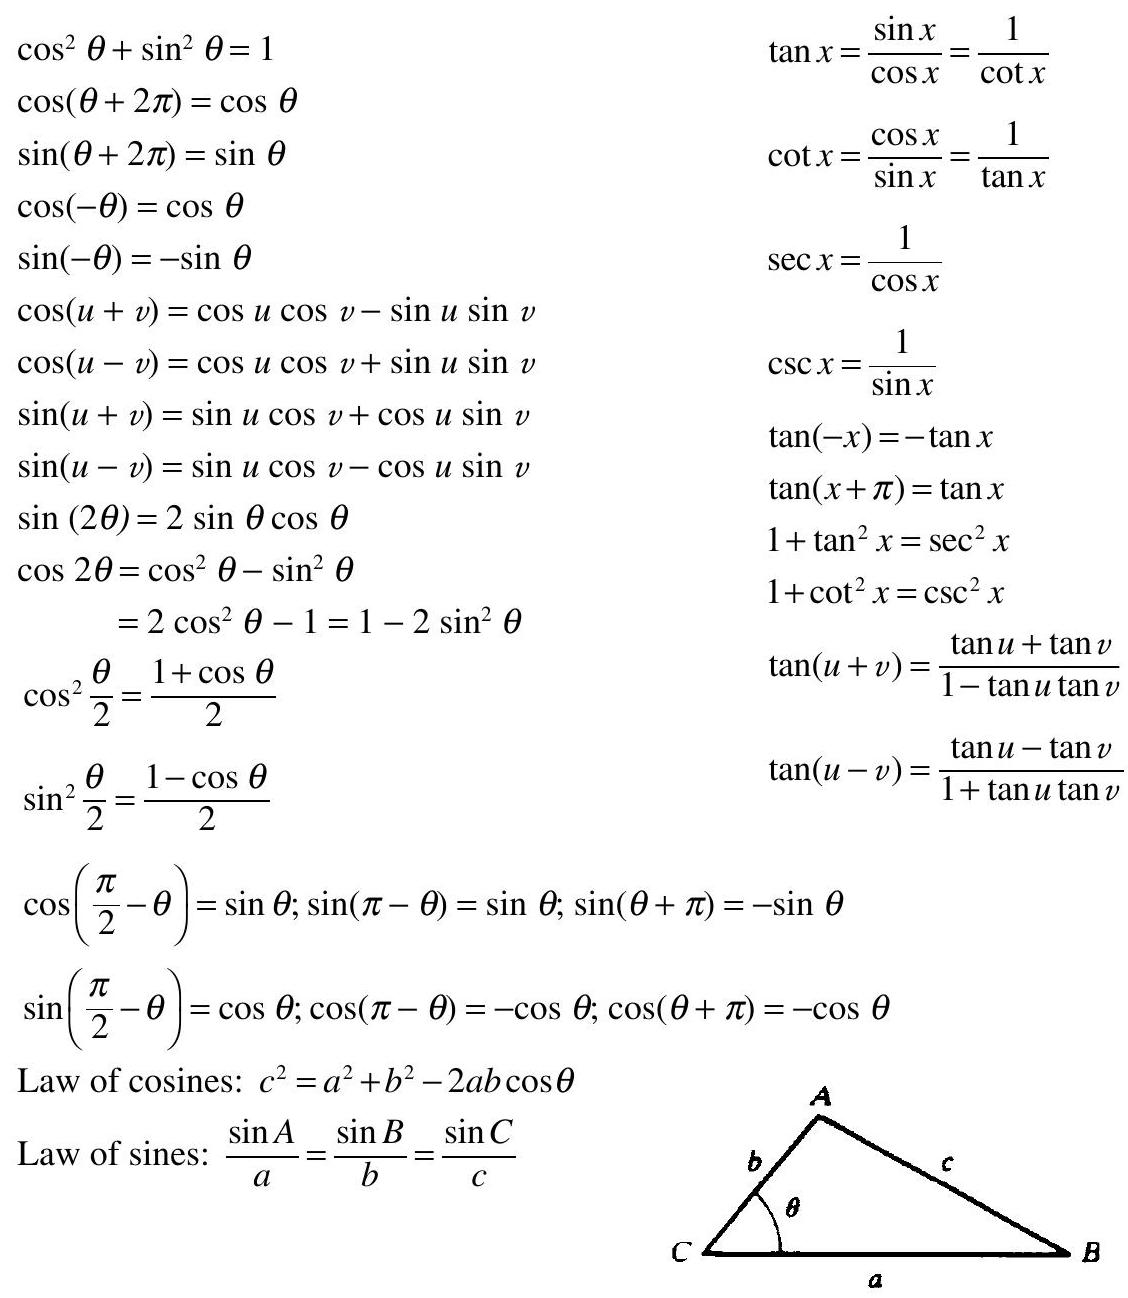
\includegraphics[max width=\textwidth]{2024_04_20_fe2e8e718cc0fcd63d1bg-29}
\end{center}

$\cos ^{2} \theta+\sin ^{2} \theta=1$

$\cos (\theta+2 \pi)=\cos \theta$

$\sin (\theta+2 \pi)=\sin \theta$

$\cos (-\theta)=\cos \theta$

$\sin (-\theta)=-\sin \theta$

$\cos (u+v)=\cos u \cos v-\sin u \sin v$

$\cos (u-v)=\cos u \cos v+\sin u \sin v$

$\sin (u+v)=\sin u \cos v+\cos u \sin v$

$\sin (u-v)=\sin u \cos v-\cos u \sin v$

$\sin (2 \theta)=2 \sin \theta \cos \theta$

$\cos 2 \theta=\cos ^{2} \theta-\sin ^{2} \theta$

$=2 \cos ^{2} \theta-1=1-2 \sin ^{2} \theta$

$\cos ^{2} \frac{\theta}{2}=\frac{1+\cos \theta}{2}$

$\sin ^{2} \frac{\theta}{2}=\frac{1-\cos \theta}{2}$

$\cos \left(\frac{\pi}{2}-\theta\right)=\sin \theta ; \sin (\pi-\theta)=\sin \theta ; \sin (\theta+\pi)=-\sin \theta$

$\sin \left(\frac{\pi}{2}-\theta\right)=\cos \theta ; \cos (\pi-\theta)=-\cos \theta ; \cos (\theta+\pi)=-\cos \theta$

Law of cosines: $c^{2}=a^{2}+b^{2}-2 a b \cos \theta$

Law of sines: $\frac{\sin A}{a}=\frac{\sin B}{b}=\frac{\sin C}{c}$ $\tan x=\frac{\sin x}{\cos x}=\frac{1}{\cot x}$

$\cot x=\frac{\cos x}{\sin x}=\frac{1}{\tan x}$

$\sec x=\frac{1}{\cos x}$

$\csc x=\frac{1}{\sin x}$

$\tan (-x)=-\tan x$

$\tan (x+\pi)=\tan x$

$1+\tan ^{2} x=\sec ^{2} x$

$1+\cot ^{2} x=\csc ^{2} x$

$\tan (u+v)=\frac{\tan u+\tan v}{1-\tan u \tan v}$

$\tan (u-v)=\frac{\tan u-\tan v}{1+\tan u \tan v}$

\section*{APPENDIX B}
\section*{Geometric Formulas}
( $A=$ area, $C=$ circumference, $V=$ volume, $S=$ lateral surface area)

\begin{center}
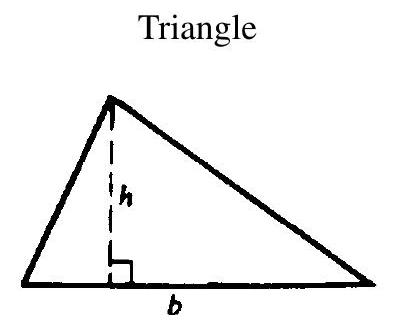
\includegraphics[max width=\textwidth]{2024_04_20_fe2e8e718cc0fcd63d1bg-30(1)}
\end{center}

$A=\frac{1}{2} b h$\\
Trapezoid

\begin{center}
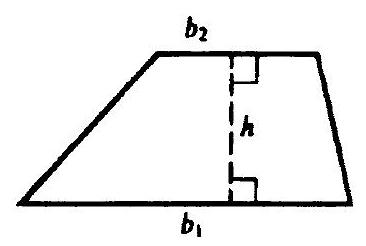
\includegraphics[max width=\textwidth]{2024_04_20_fe2e8e718cc0fcd63d1bg-30(4)}
\end{center}

$A=\frac{1}{2}\left(b_{1}+b_{2}\right) h$\\
Parallelogram

\begin{center}
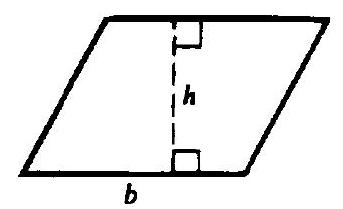
\includegraphics[max width=\textwidth]{2024_04_20_fe2e8e718cc0fcd63d1bg-30(2)}
\end{center}

$A=b h$\\
Circle

\begin{center}
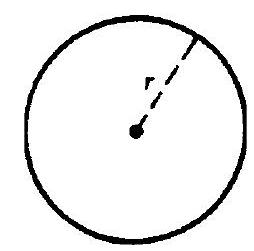
\includegraphics[max width=\textwidth]{2024_04_20_fe2e8e718cc0fcd63d1bg-30(5)}
\end{center}

$a=\pi r^{2}, C=2 \pi r$\\
Sphere

\begin{center}
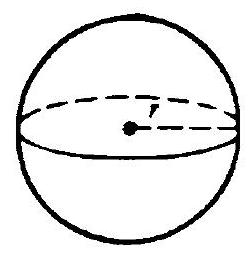
\includegraphics[max width=\textwidth]{2024_04_20_fe2e8e718cc0fcd63d1bg-30(3)}
\end{center}

$V=\frac{4}{3} \pi r^{3}$\\
$S=4 \pi r^{2}$\\
Cone

\begin{center}
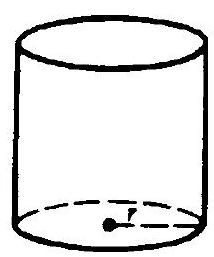
\includegraphics[max width=\textwidth]{2024_04_20_fe2e8e718cc0fcd63d1bg-30}
\end{center}

$V=\pi r^{2} h$\\
$S=2 \pi r h$

$V=\frac{1}{3} \pi r^{2} h$

$S=\pi r s=\pi r \sqrt{r^{2}+h^{2}}$

\section*{Index}
\section*{A}
Abel's theorem, 386

Abscissa, 9

Absolute maximum and minimum, 107, 453

Absolute value, 1

Absolutely convergent series, 376

Acceleration:

angular, 163

in curvilinear motion, 332

in rectilinear motion, 161

tangential and normal components of, 333

vector, 332

Alternating:

harmonic series, 376

series, 375

theorem, 375

Amplitude, 141

Analytic proofs of geometric theorems, 13

Angle:

between two curves, 144, 342

measure, 130

of inclination, 144, 341

Angular velocity and acceleration, 163

Antiderivative, 181

Approximation by differentials, 174

Approximation by series, 398

Arc length, 237, 308

derivative of, 312,343

formula, 238

Area:

between curves, 236

by integration, 190, 481

in polar coordinates, 351,520

of a curved surface, 489

of a surface of revolution, 301

under a curve, 190

Argument, 49

Asymptote, 120

of hyperbola, 39

Average rate of change, 73

Average value of a function, 198

Average velocity, 161

Axis of revolution, 244

Axis of symmetry, 120

of a parabola, 37

\section*{B}
Binomial series, 399

Binormal vector, 461

Bliss's theorem, 305

Bounded sequence, 353

Bounded set in a plane, 453\\
C

Carbon dating, 232

Cardioid, 340

Catenary, 220

Center of curvature, 314

Center of mass, 510

Center:

of a hyperbola, 43

of an ellipse, 42

Centroid:

of a plane region, 481

of a volume, 500

Chain rule, 80, 415

Change of variables in an integral, 199

Circle, 29

equation of, 29

of curvature, 313

osculating, 313

Circular motion, 163

Closed interval, 2

Closed set, 453

Comparison test, 367

Complement, 453

Complementary function, 517

Completing the square, 30

Components of a vector, 322

Composite function, 80

Composition, 80

Compound interest, 221, 232

Concave upward, downward, 119

Concavity, 119

Conditionally convergent series, 376

Cone, elliptic, 443

Conic sections, 39

Conjugate axis of a hyperbola, 43

Continuous function, 66, 68, 405

on [a,b], 68

on the left (right), 68

Convergence of series, 360

absolute, conditional, 376

Convergence, uniform, 385

Convergent sequence, 352

Coordinate, 1

axes, 9

Coordinate system:

cylindrical and spherical, 498

linear, 1

rectangular, 9

right-handed, 426

polar, 133, 339

Cosecant, 142

Cosine, 131

Cosine (Cont.):

direction cosines, 428

Cotangent, 142

Critical numbers, 105

Cross product of vectors, 428

Cross-section formula, 248

Cubic curve, 39

Curl, 465

Curvature, 313

of a polar curve, 343

Curve sketching, 122

Curvilinear motion, 332

Cycloid, 315

Cylindrical coordinates, 498

Cylindrical shell formula, 247

Cylindrical surfaces, 441

D

Decay constant, 230

Decreasing:

function, 100

sequence, 354

Definite integral, 192

Degree, 130

Del, 464

Deleted disk, 405

Delta neighborhood, 4

Delta notation, 73

Density, 510

Dependent variable, 49

Derivative, 73

directional, 452

first, 62

higher order, 82,90

of a vector function, 324

of arc length, 312,343

of inverse functions, 81

partial, 405

second, 82

third, 82

Determinants, 428

Difference of shells formula, 247

Difference rule for derivatives, 79

Differentiability, 74, 415

Differential, 174

total, 414

Differential equation, 516

linear, of the first order, 517

order of a, 516

second order, 517

separable, 516

solution (general) of a, 516

Differentiation, 79

formulas, 79

implicit, 90, 417

logarithmic, 210

of inverse functions, 81

of power series, 385

of trigonometric functions, 139

of vector functions, 324, 460\\
Directed angles, 131

Direction cosines, 428

Direction numbers, 431

Directional derivative, 452

Directrix of a parabola, 41

Discontinuity, 66

jump, 67

removable, 66

Disk:

deleted, 405

open, 405

Disk formula, 244

Displacement, 74

Distance formula, 11

for polar coordinates, 351

Divergence (div):

of a sequence, 352

of a series, 360

of a vector function, 464

Divergence theorem, 362

Domain of a function, 49

Dot product of vectors, 323

Double integral, 474, 489

E

e, 215

$e^{x}, 214$

Eccentricity

of an ellipse, 42

of a hyperbola, 43

Ellipses, 38

center, eccentricity, foci, major axis, minor axis of, 42

Ellipsoid, 442

Elliptic:

cone, 443

paraboloid, 442

Equations, graphs of, 37

Equilateral hyperbola, 46

Even functions, 122

Evolute, 314

Exponential functions, 214, 216

Exponential growth and decay, 230

Extended law of the mean, 100

Extreme Value Theorem, 69

Extremum, relative, 98

First derivative, 62

First derivative test, 106

First octant, 426

Foci:

of an ellipse, 42

of a hyperbola, 43

Focus of a parabola, 41

Free fall, 162

Frequency, 141

Function, 49

composite, 80

continuous, 405

Function (Cont.)

decreasing, 100

differentiable, 74, 415

domain of a, 49

even, 122

exponential, 214, 216

homogeneous, 516

hyperbolic, 220

implicit, 90

increasing, 100

integrable, 192

inverse, 81

inverse trigonometric, 152

logarithmic, 206

odd, 122

of several variables, 405

one-to-one, 81

range of a, 49

trigonometric, 139

Fundamental Theorem of Calculus, 199

\section*{G}
Gamma function, 300

General exponential function, 216

General logarithmic functions, 217

Generalized Rolle's theorem, 99

Geometric series, 360

Gradient, 453, 464

Graphs of equations, 20, 37

Graphs of functions, 122

Gravity, 162

Growth constant, 230

\section*{H}
Half-life, 231

Half-open interval, 3

Harmonic series, 362

Higher order: derivatives, 90

partial derivatives, 407

Higher order law of the mean, 100

Homogeneous:

bodies, 510

equation, ???

function, 516

Horizontal asymptote, 120

Hyperbola, 38,43

asymptotes of, 39

center, conjugate axes, eccentricity,

foci, tranverse axes, vertices

equilateral, 43,46

Hyperbolic functions, 220

Hyperbolic paraboloid, 443

Hyperboloid:

of one sheet, 443

of two sheets, 444

\section*{I}
Implicit differentiation, 90, 417

Implicit functions, 90\\
Improper integrals, 293

Increasing

function, 100

sequence, 354

Indefinite integral, 181

Independent variable, 49

Indeterminate types, 223

Inequalities, 3

Infinite intervals, 3

Infinite limit, 57

of integration, 293

Infinite sequence, 352

limit of, 352

Infinite series, 360

Inflection point, 120

Initial position, 162

Initial velocity, 162

Instantaneous rate of change, 73

Instantaneous velocity, 161

Integrable, 192

Integral:

definite, 192

double, 474

improper, 293

indefinite, 181

iterated, 475

line, 466

Riemann, 192

test for convergence, 366

triple, 499

Integrand, 181

Integrating factor, 516

Integration:

by miscellaneous substitutions, 288

by partial fractions, 279

by parts, 259

by substitution, 182

by trigonometric substitution, 268

of power series, 385

plane area by double, 481

Intercepts, 21

Intermediate Value Theorem, 69

Interval of convergence, 383

Intervals, 2

Inverse cosecant, 155

Inverse cosine, 153

Inverse cotangent, 154

Inverse function, 81

Inverse secant, 155

Inverse sine, 152

Inverse tangent, 153

Inverse trigonometric functions, 152

Irreducible polynomial, 279

Iterated integral, 475

\section*{J}
Jump discontinuity, 67

L

Latus rectum of a parabola, 41

Law of cosines, 134

Law of sines, 134

Law of the mean, 99

Extended, 100

Higher-order, 100

Lemniscate, 340

Length of arc, 130

L'Hôpital's Rule, 222

Limaçon, 340

Limit

infinite, 57

of a function, 56,405

of a sequence, 352

right and left, 57

Limit comparison test, 367

Line, 18

equation of a, 20

in space, 431

slope of a, 18

Line integral, 466

Linear coordinate system, 1

Linear differential equation of the first order, 517

Logarithm, natural, 206

Logarithmic differentiation, 210

Logarithmic functions, 217

Lower limit of an integral, 192

\section*{M}
Maclaurin series, 396

Major axis of an ellipse, 42

Mass, 510

Maximum and minimum:

absolute, 107

relative, 98

Mean-Value theorem for derivatives, 99

Mean-Value theorem for integrals, 198

Midpoint formulas, 12

Minor axis of an ellipse, 42

Midpoint rule for integrals, 204

Moment of inertia:

of planar mass, 510

of planar region, 482

of a volume, 500

Monotonic sequence, 354

Motion:

circular, 163

curvilinear, 332

rectilinear, 161

Motion under the influence of gravity, 162

\section*{$\mathbf{N}$}
Natural logarithm, 206

Newton's law of cooling, 232

Newton's method, 175

Nondecreasing (nonincreasing) sequence, 354

Normal component of acceleration, 333

Normal line to a plane curve, 94

Normal line to a surface, 445

Normal plane to a space curve, 445, 461

\section*{O}
Octants, 426

One-to-one function, 81

Open disk, 405

Open interval, 2

Open set, 415

Ordinate, 9

Origin, 1

Osculating circle, 313

Osculating plane, 461

Pappus, theorem of, 488

Parabola, 37

focus, directrix, latus rectum, vertex, 41

Paraboloid:

elliptic, 442

hyperbolic, 443

Paradox, Zeno's, 364

Parallel lines, slopes of, 22

Parameter, 307

Parametric equations, 307

for surfaces, 462

Partial derivative, 405

higher order, 407

Partial fractions, 279

Partial sums of a series, 360

Particular solution, 517

Period, 141

Perpendicular lines, slopes of, 22

Plane, 432

vectors, 321

Point of inflection, 120

Point-slope equation of a line, 21

Polar axis, 339

Polar coordinates, 133, 339, 340

Polar curves, 340

Polar equation, 339

Pole, 339

Position vector, 324, 426

Positive series, 366

Positive $x$ axis, $y$ axis, 9

Power chain rule, 84

Power rule for derivatives, 79

Power series, 383

differentiation of, 385

integration of, 385

interval of convergence of, 383

radius of convergence of, 384

uniform convergence of, 385

p-series, 368

Principal normal, 461

Product rule for derivatives, 79

\section*{Q}
Quadrants, 10

Quick formula I, 182

Quick formula II, 208

Quotient rule for derivatives, 79

\section*{R}
Radian measure, 130

Radius of convergence, 383

Radius of curvature, 313

Radius vector, 324

Range of a function, 49

Rate of change, 73

Ratio of a geometric series, 360

Ratio test, 376

Rational function, 68, 279

Rectangular coordinate system, 9

Rectifying plane, 461

Rectilinear motion, 161

Reduction formulas, 263-264

Related rates, 167

Relative extrema (maximum and minimum), 98, 105, 106, 453

Remainder term, 397

Removable discontinuity, 70

Riemann integral, 192

Riemann sum, 192

Right-handed system, 426

Rolle's theorem, 98

generalized, 99

Root test, 376

Rose with three petals, 340

\section*{S}
Scalar product of vectors, 323

Scalars, 321

Secant function, 142

Second derivative, 82

Second derivative test, 105

Semimajor (semiminor) axis of an ellipse, 42

Separable differential equation, 516

Sequences:

bounded, 353

convergent and divergent, 352

limit of, 352

decreasing, increasing, nondecreasing,

nonincreasing, monotonic, 354

Series, infinite, 360

absolutely convergent, 376

alternating, 375

binomial, 399

conditionally convergent, 376

convergent and divergent, 360

geometric, 360

harmonic, 362

Maclaurin, 396

partial sums of, 360

positive, 366

power, 383

p-series, 368

remainder after $n$ terms of a, 397

Taylor, 396

sum of, 360

terms of, 360

with positive terms, 366\\
Sigma notation, 190

Simpson's rule, 204

Sine, 131

Slicing formula, 248

Slope of a line, 18

Slopes:

of parallel lines, 22

of perpendicular lines, 22

Slope-intercept equation of a line, 21

Solid of revolution, 244

Space curve, 445,461

Space vectors, 426

Speed, 332

Sphere, 441

Spherical coordinates, 498

Squeeze theorem, 353

Standard equation of a circle, 29

Standing still, 162

Substitution method, 182

Sum of a series, 360

Sum rule for derivatives, 79

Surfaces, 462

cylindrical, 441

Surface of revolution, 301, 446

Symmetry, 120, 122

axis of, 37,120

T

Tabular method for absolute extrema, 107

Tangent function, 142

Tangent line to a plane curve, 93

Tangent line to a space curve, 445

Tangent plane to a surface, 445

Tangential component of acceleration, 333

Taylor series, 396

Taylor's formula with remainder, 397

Terms of a series, 360

Third derivative, 82

Total differential, 414

Transverse axis of a hyperbola, 43

Trapezoidal rule, 202

Triangle inequality, 2

Trigonometric functions, 131, 140, 142

Trigonometric integrands, 266

Trigonometric substitutions, 268

Trigonometry review, 130

Triple integral, 499

Triple scalar product, 430

Triple vector product, 431

U

Uniform convergence, 385

Unit normal to a surface, 463

Unit tangent vector, 325

Upper limit of an integral, 192

V

Vector:

equation of a line, 431

equation of a plane, 432

Vector (Cont.):

position, 324, 426

product, 428

projections, 324

radius, 324

unit, 322

unit tangent, 325

velocity, 332

zero, 321

Vector functions, 324

curl of, 465

differentiation of, 324. 460

divergence of, 464

integration of, 465

Vectors, 321

acceleration, 332

addition of, 321

components of, 322

cross product of, 428

difference of, 322

direction cosines of, 428

dot product of, 323

magnitude of, 321

plane, 321

scalar product of, 323

scalar projection of, 324

space, 426

sum of, 321

triple scalar product of, 430

triple vector product of, 431

vector product of, 428

vector projection of, 324

Velocity:

angular, 163

average, 161\\
Velocity (Cont.):

in curvilinear motion, 332

in rectilinear motion, 161

initial, 162

instantaneous, 161

vector, 332

Vertex of a parabola, 41

Vertical asymptote, 120

Vertices:

of a hyperbola, 43

of an ellipse, 42

Volume:

given by an iterated integral, 475

of solids of revolution, 244

under a surface, 489

with area of cross section given, 248

W

Washer formula, 246

Work done by a force, 329

\section*{$\mathbf{X}$}
$x$ axis, 9

positive, 9

$x$ coordinate, 9

\section*{$\mathbf{Y}$}
$y$ axis, 9

positive, 9

$y$ coordinate, 9

$y$ intercept, 21

Z

Zeno's paradox, 364

Zero vector, 321


\end{document}